%!TEX root = ../main.tex
\chapter{Corrente elettrica nei conduttori}

\section{Fenomeni di conduzione di carica elettrica}

Ritorniamo ai materiali conduttori in equilibrio elettrostatico. Abbiamo visto che in tali condizioni le eventuali cariche in eccesso sono depositate solo sulla superficie, all'interno il campo elettrico è nullo e la densità di carica libera anche essa è zero. Per ogni elettrone c'è un nucleo positivo vicino che lo neutralizza, non c'è squilibrio di cariche, inoltre esse all'equilibrio sono in quiete. Questo concetto ha senso solo dal punto di vista statistico. Se consideriamo un pezzettino di conduttore, all'equilibrio avremo tante cariche negative che si muovono in modo casuale secondo un moto di agitazione termica molto simile a quello che abbiamo in un gas di molecole. Se calcoliamo il valore medio della velocità vettoriale, anche prendendo un piccolissimo volume, avremo che essa è zero. Questo accade perché per ogni elettrone che si muove in una direzione c'è ne è sicuramente un altro che si muove in direzione opposta.

\[
	\langle \vec{v} \rangle = \frac{\sum_i \vec{v}_i}{N}
\]

Dal punto di vista concettuale, questo ci comunica che non esiste una direzione di moto preferenziale per gli elettroni. In realtà, anche in un volume piccolissimo, essi sono numerosi e hanno una certa velocità. Nel rame e nell'argento, la densità di elettroni per unità di volume è dell'ordine di $10^{28}/m^3$; l'ordine di grandezza è lo stesso per tutti i conduttori metallici. Capiamo quindi Che s proviamo a calcolare la velocità quadratica media, questa è ben lontana dall'essere pari a $0$.

\[
	\overline{v} = \sqrt{\langle v^2 \rangle}
\]

A $300 K$, la velocità quadratica media è $120\,km/s$.

\begin{figure}[htpb]
	\centering

	% Pattern Info
	 
	\tikzset{
	pattern size/.store in=\mcSize, 
	pattern size = 5pt,
	pattern thickness/.store in=\mcThickness, 
	pattern thickness = 0.3pt,
	pattern radius/.store in=\mcRadius, 
	pattern radius = 1pt}
	\makeatletter
	\pgfutil@ifundefined{pgf@pattern@name@_7pir68r1b}{
	\pgfdeclarepatternformonly[\mcThickness,\mcSize]{_7pir68r1b}
	{\pgfqpoint{0pt}{0pt}}
	{\pgfpoint{\mcSize+\mcThickness}{\mcSize+\mcThickness}}
	{\pgfpoint{\mcSize}{\mcSize}}
	{
	\pgfsetcolor{\tikz@pattern@color}
	\pgfsetlinewidth{\mcThickness}
	\pgfpathmoveto{\pgfqpoint{0pt}{0pt}}
	\pgfpathlineto{\pgfpoint{\mcSize+\mcThickness}{\mcSize+\mcThickness}}
	\pgfusepath{stroke}
	}}
	\makeatother

	% Pattern Info
	 
	\tikzset{
	pattern size/.store in=\mcSize, 
	pattern size = 5pt,
	pattern thickness/.store in=\mcThickness, 
	pattern thickness = 0.3pt,
	pattern radius/.store in=\mcRadius, 
	pattern radius = 1pt}
	\makeatletter
	\pgfutil@ifundefined{pgf@pattern@name@_9503dhk18}{
	\pgfdeclarepatternformonly[\mcThickness,\mcSize]{_9503dhk18}
	{\pgfqpoint{0pt}{0pt}}
	{\pgfpoint{\mcSize+\mcThickness}{\mcSize+\mcThickness}}
	{\pgfpoint{\mcSize}{\mcSize}}
	{
	\pgfsetcolor{\tikz@pattern@color}
	\pgfsetlinewidth{\mcThickness}
	\pgfpathmoveto{\pgfqpoint{0pt}{0pt}}
	\pgfpathlineto{\pgfpoint{\mcSize+\mcThickness}{\mcSize+\mcThickness}}
	\pgfusepath{stroke}
	}}
	\makeatother
	\tikzset{every picture/.style={line width=0.75pt}} %set default line width to 0.75pt        

	\begin{tikzpicture}[x=0.75pt,y=0.75pt,yscale=-0.7,xscale=0.7]
	%uncomment if require: \path (0,300); %set diagram left start at 0, and has height of 300

	%Shape: Circle [id:dp9219367414045321] 
	\draw  [pattern=_7pir68r1b,pattern size=6pt,pattern thickness=0.75pt,pattern radius=0pt, pattern color={rgb, 255:red, 222; green, 222; blue, 222}] (95,164.25) .. controls (95,109.44) and (139.44,65) .. (194.25,65) .. controls (249.06,65) and (293.5,109.44) .. (293.5,164.25) .. controls (293.5,219.06) and (249.06,263.5) .. (194.25,263.5) .. controls (139.44,263.5) and (95,219.06) .. (95,164.25) -- cycle ;
	%Shape: Ellipse [id:dp8917923509185433] 
	\draw  [pattern=_9503dhk18,pattern size=6pt,pattern thickness=0.75pt,pattern radius=0pt, pattern color={rgb, 255:red, 222; green, 222; blue, 222}] (468.57,161.56) .. controls (468.57,132.03) and (492.5,108.09) .. (522.03,108.09) .. controls (551.56,108.09) and (575.5,132.03) .. (575.5,161.56) .. controls (575.5,191.09) and (551.56,215.02) .. (522.03,215.02) .. controls (492.5,215.02) and (468.57,191.09) .. (468.57,161.56) -- cycle ;
	%Curve Lines [id:da025791305803244624] 
	\draw [line width=2.25]    (293.5,164.25) .. controls (356.5,77) and (418.5,249) .. (468.57,161.56) ;
	%Curve Lines [id:da0029303514799270403] 
	\draw    (334,130) .. controls (373.2,127.55) and (377.83,151.51) .. (413.76,166.59) ;
	\draw [shift={(416,167.5)}, rotate = 201.54] [fill={rgb, 255:red, 0; green, 0; blue, 0 }  ][line width=0.08]  [draw opacity=0] (10.72,-5.15) -- (0,0) -- (10.72,5.15) -- (7.12,0) -- cycle    ;
	%Curve Lines [id:da8872938466077263] 
	\draw    (373.67,170.83) .. controls (382.13,177.1) and (395.89,187.2) .. (409.69,192.81) ;
	\draw [shift={(412.33,193.83)}, rotate = 199.98] [fill={rgb, 255:red, 0; green, 0; blue, 0 }  ][line width=0.08]  [draw opacity=0] (10.72,-5.15) -- (0,0) -- (10.72,5.15) -- (7.12,0) -- cycle    ;

	% Text Node
	\draw (194.25,55) node    {$+$};
	% Text Node
	\draw (194.25,275) node    {$+$};
	% Text Node
	\draw (304.25,165) node    {$+$};
	% Text Node
	\draw (84.25,165) node    {$+$};
	% Text Node
	\draw (272.03,87.22) node    {$+$};
	% Text Node
	\draw (116.47,242.78) node    {$+$};
	% Text Node
	\draw (272.03,242.78) node    {$+$};
	% Text Node
	\draw (116.47,87.22) node    {$+$};
	% Text Node
	\draw (237.23,63.74) node    {$+$};
	% Text Node
	\draw (151.27,266.26) node    {$+$};
	% Text Node
	\draw (295.51,207.98) node    {$+$};
	% Text Node
	\draw (92.99,122.02) node    {$+$};
	% Text Node
	\draw (296.24,123.79) node    {$+$};
	% Text Node
	\draw (92.26,206.21) node    {$+$};
	% Text Node
	\draw (235.46,266.99) node    {$+$};
	% Text Node
	\draw (153.04,63.01) node    {$+$};
	% Text Node
	\draw (283.56,55.41) node    {$V_{1}$};
	% Text Node
	\draw (522.03,96.2) node    {$+$};
	% Text Node
	\draw (522.03,225.8) node    {$+$};
	% Text Node
	\draw (586.84,161) node    {$+$};
	% Text Node
	\draw (457.23,161) node    {$+$};
	% Text Node
	\draw (567.86,115.18) node    {$+$};
	% Text Node
	\draw (476.21,206.82) node    {$+$};
	% Text Node
	\draw (567.86,206.82) node    {$+$};
	% Text Node
	\draw (476.21,115.18) node    {$+$};
	% Text Node
	\draw (547.35,101.35) node    {$+$};
	% Text Node
	\draw (496.71,220.65) node    {$+$};
	% Text Node
	\draw (581.68,186.32) node    {$+$};
	% Text Node
	\draw (462.38,135.68) node    {$+$};
	% Text Node
	\draw (582.12,136.72) node    {$+$};
	% Text Node
	\draw (461.95,185.28) node    {$+$};
	% Text Node
	\draw (546.31,221.08) node    {$+$};
	% Text Node
	\draw (497.76,100.92) node    {$+$};
	% Text Node
	\draw (626.18,100.98) node    {$V_{2} < V_{1}$};
	% Text Node
	\draw (386.56,125.41) node    {$\vec{E}$};
	% Text Node
	\draw (366.38,163.68) node    {$+$};

	\end{tikzpicture}
\end{figure}
\FloatBarrier

Immaginiamo di avere due conduttori inizialmente in equilibrio elettrostatico che si trovano a due potenziali elettrostatici differenti $V_1$ e $V_2$. Se li colleghiamo con un filo di materiale conduttore, accade che all'interno di esso apparirà un campo elettrico. Le cariche cominciano a spostarsi da un conduttore all'altro. Il fenomeno è detto di \textbf{conduzione} di carica elettrica, o trasporto. Quando abbiamo un moto ordinato di cariche in una certa direzione, diciamo che in quel conduttore è presente una \textbf{corrente elettrica}. Questo processo di moto di cariche è transitorio e terminerà quando i potenziali Dei conduttori saranno uguali. La corrente elettrica in questo caso specifico dura per un tempo molto limitato che impedisce l'esecuzione di studi sistematici del fenomeno.

I fenomeni di conduzione di carica per questo sono rimasti inesplorati fino all'800, in cui Alessandro Volta inventò il \textbf{generatore di forza elettromotrice}.
Si tratta di un dispositivo in grado di mantenere una differenza di potenziale costante fra due conduttori a contatto. Così facendo il flusso di elettroni può durare per molto più tempo e quindi nel conduttore si instaura una corrente elettrica stabile, in un regime di equilibrio dinamico e non più di equilibrio elettrostatico. Nella sua versione originale la pila di Volt o cella voltaica consta di una serie di elementi ciascuno dei quali è costituito da un disco di zinco, un tampone imbevuto di una soluzione acquosa di acido solforico e un disco di rame. Esso risulta carico positivamente e quello di zinco negativamente. Se si misura con uno strumento elettrostatico la d.d.p. tra i due dischi si trova un valore fisso caratteristico della coppia di metalli che è detto $fem$ della pila. Collegando alle estremità della pila un conduttore, ad esempio un filo metallico, viene stabilita in questo una corrente elettrica costante nel tempo, denominata come corrente continua. In realtà con una pila di Volta la corrente diminuisce molto lentamente nel tempo.

Immaginiamo di collegare il nostro generatore di forza elettromotrice ad un oggetto costituito da materiale conduttore. Inizierà ad esserci un flusso ordinato di cariche elettriche dovuto al campo elettrico prodotto dal generatore.

\begin{figure}[htpb]
	\centering

	\tikzset{every picture/.style={line width=0.75pt}} %set default line width to 0.75pt        

	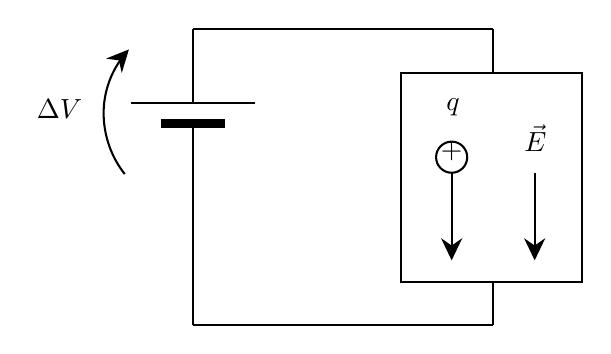
\begin{tikzpicture}[x=0.75pt,y=0.75pt,yscale=-1,xscale=1]
	%uncomment if require: \path (0,300); %set diagram left start at 0, and has height of 300

	%Shape: Battery [id:dp7947896056729546] 
	\draw  [fill={rgb, 255:red, 0; green, 0; blue, 0 }  ,fill opacity=1 ] (148.3,130.4) -- (148.3,94.4) (118.3,86.4) -- (178.3,86.4) (148.3,86.4) -- (148.3,50.4) (133.3,97.6) -- (133.3,94.4) -- (163.3,94.4) -- (163.3,97.6) -- (133.3,97.6) -- cycle ;
	%Straight Lines [id:da8636566827035768] 
	\draw    (148.3,50.4) -- (292.8,50.4) ;
	%Shape: Rectangle [id:dp5030241254746104] 
	\draw   (248.7,71.6) -- (335.8,71.6) -- (335.8,172.6) -- (248.7,172.6) -- cycle ;
	%Shape: Circle [id:dp11503800279281395] 
	\draw   (265.4,112.3) .. controls (265.4,108.16) and (268.76,104.8) .. (272.9,104.8) .. controls (277.04,104.8) and (280.4,108.16) .. (280.4,112.3) .. controls (280.4,116.44) and (277.04,119.8) .. (272.9,119.8) .. controls (268.76,119.8) and (265.4,116.44) .. (265.4,112.3) -- cycle ;

	%Straight Lines [id:da5166399090598475] 
	\draw    (272.9,119.8) -- (272.9,159) ;
	\draw [shift={(272.9,162)}, rotate = 270] [fill={rgb, 255:red, 0; green, 0; blue, 0 }  ][line width=0.08]  [draw opacity=0] (10.72,-5.15) -- (0,0) -- (10.72,5.15) -- (7.12,0) -- cycle    ;
	%Straight Lines [id:da10335817060324226] 
	\draw    (312.9,119.8) -- (312.9,159) ;
	\draw [shift={(312.9,162)}, rotate = 270] [fill={rgb, 255:red, 0; green, 0; blue, 0 }  ][line width=0.08]  [draw opacity=0] (10.72,-5.15) -- (0,0) -- (10.72,5.15) -- (7.12,0) -- cycle    ;
	%Straight Lines [id:da9745597516547506] 
	\draw    (292.8,71.2) -- (292.8,50.4) ;
	%Straight Lines [id:da9311759273417342] 
	\draw    (292.8,193.2) -- (292.8,172.4) ;
	%Straight Lines [id:da04193895564665562] 
	\draw    (148.3,193.2) -- (292.8,193.2) ;
	%Straight Lines [id:da4895770815624165] 
	\draw    (148.3,193.2) -- (148.3,130.4) ;
	%Curve Lines [id:da18786427144500872] 
	\draw    (115.4,120.4) .. controls (103.63,105.73) and (100.05,81.38) .. (115.63,62.44) ;
	\draw [shift={(117.4,60.4)}, rotate = 492.51] [fill={rgb, 255:red, 0; green, 0; blue, 0 }  ][line width=0.08]  [draw opacity=0] (10.72,-5.15) -- (0,0) -- (10.72,5.15) -- (7.12,0) -- cycle    ;

	% Text Node
	\draw (272.9,109.8) node    {$+$};
	% Text Node
	\draw (273.6,88.2) node    {$q$};
	% Text Node
	\draw (313.2,103) node    {$\vec{E}$};
	% Text Node
	\draw (84,89) node    {$\Delta V$};

	\end{tikzpicture}
\end{figure}
\FloatBarrier

\textbf{Osservazione.} \emph{In un metallo gli unici sul 9 portatori di carica sono gli elettroni, ma sappiamo che in altri casi, come la pila o il plasma, le cariche possono anche essere positive.}
Il flusso che ci aspettiamo è la combinazione di un moto caotico a velocità elevatissima sovrapposto a un moto molto lento detto di deriva delle cariche nella direzione del campo elettrico $\vec{E}$. Non ci concentreremo sulla velocità microscopica di ciascun elettrone ma solo su questa \emph{velocità di deriva}, $ v_d  $. In questo caso il valore medio delle velocità degli elettroni non sarà più zero, ma sarà uguale a $v_d (0.15\,mm/s)$. Vediamo quindi come la perturbazione introdotta dalla conduzione sulla velocità dell'elettrone sia molto piccola.

\[
	\langle \vec{v} \rangle = \vec{v}_d
\]

Abbiamo quindi il nostro conduttore, al cui interno è presente un campo elettrico e le cui cariche positive si muovono per questo a una certa velocità di deriva $ v_d  $. Siamo in grado di calcolarla in tutti i punti del conduttore in maniera precisa, definendo il campo vettoriale:

\[
	\vec{v}_d = \vec{v}_d(x,y,z)
\]

\begin{figure}[htpb]
	\centering

	% Pattern Info
	 
	\tikzset{
	pattern size/.store in=\mcSize, 
	pattern size = 5pt,
	pattern thickness/.store in=\mcThickness, 
	pattern thickness = 0.3pt,
	pattern radius/.store in=\mcRadius, 
	pattern radius = 1pt}
	\makeatletter
	\pgfutil@ifundefined{pgf@pattern@name@_3zx8u6z0b}{
	\pgfdeclarepatternformonly[\mcThickness,\mcSize]{_3zx8u6z0b}
	{\pgfqpoint{0pt}{0pt}}
	{\pgfpoint{\mcSize+\mcThickness}{\mcSize+\mcThickness}}
	{\pgfpoint{\mcSize}{\mcSize}}
	{
	\pgfsetcolor{\tikz@pattern@color}
	\pgfsetlinewidth{\mcThickness}
	\pgfpathmoveto{\pgfqpoint{0pt}{0pt}}
	\pgfpathlineto{\pgfpoint{\mcSize+\mcThickness}{\mcSize+\mcThickness}}
	\pgfusepath{stroke}
	}}
	\makeatother
	\tikzset{every picture/.style={line width=0.75pt}} %set default line width to 0.75pt        

	\begin{tikzpicture}[x=0.75pt,y=0.75pt,yscale=-1,xscale=1]
	%uncomment if require: \path (0,321); %set diagram left start at 0, and has height of 321

	%Shape: Ellipse [id:dp6145612949263457] 
	\draw   (356.94,221.86) .. controls (342.78,213.69) and (342.9,186.98) .. (357.2,162.2) .. controls (371.51,137.43) and (394.58,123.97) .. (408.74,132.14) .. controls (422.89,140.31) and (422.77,167.02) .. (408.47,191.8) .. controls (394.17,216.57) and (371.09,230.03) .. (356.94,221.86) -- cycle ;
	%Straight Lines [id:da5353682425174289] 
	\draw    (364.34,224.08) -- (155.66,224.08) ;
	%Curve Lines [id:da42914586957077305] 
	\draw  [dash pattern={on 0.84pt off 2.51pt}]  (194.16,130.08) .. controls (229.91,144.25) and (195.41,223.75) .. (155.66,224.08) ;
	%Straight Lines [id:da08156155803614062] 
	\draw    (402.84,130.08) -- (194.16,130.08) ;
	%Curve Lines [id:da8302824113941996] 
	\draw    (194.16,130.08) .. controls (149.41,130.25) and (112.91,219.25) .. (155.66,224.08) ;
	%Straight Lines [id:da707902971274881] 
	\draw    (469.34,177) -- (382.84,177) ;
	\draw [shift={(472.34,177)}, rotate = 180] [fill={rgb, 255:red, 0; green, 0; blue, 0 }  ][line width=0.08]  [draw opacity=0] (10.72,-5.15) -- (0,0) -- (10.72,5.15) -- (7.12,0) -- cycle    ;
	%Straight Lines [id:da9219809989976684] 
	\draw    (457.75,220.25) -- (382.84,177) ;
	\draw [shift={(460.35,221.75)}, rotate = 210] [fill={rgb, 255:red, 0; green, 0; blue, 0 }  ][line width=0.08]  [draw opacity=0] (10.72,-5.15) -- (0,0) -- (10.72,5.15) -- (7.12,0) -- cycle    ;
	%Shape: Arc [id:dp7521632869570065] 
	\draw  [draw opacity=0] (422.59,176.76) .. controls (422.59,176.84) and (422.59,176.92) .. (422.59,177) .. controls (422.59,184.13) and (420.71,190.83) .. (417.41,196.62) -- (382.84,177) -- cycle ; \draw   (422.59,176.76) .. controls (422.59,176.84) and (422.59,176.92) .. (422.59,177) .. controls (422.59,184.13) and (420.71,190.83) .. (417.41,196.62) ;
	%Shape: Ellipse [id:dp32703450933859113] 
	\draw  [pattern=_3zx8u6z0b,pattern size=6pt,pattern thickness=0.75pt,pattern radius=0pt, pattern color={rgb, 255:red, 222; green, 222; blue, 222}] (251.59,130.25) .. controls (266.43,130.25) and (278.45,151.29) .. (278.45,177.25) .. controls (278.45,203.21) and (266.43,224.25) .. (251.59,224.25) .. controls (236.76,224.25) and (224.74,203.21) .. (224.74,177.25) .. controls (224.74,151.29) and (236.76,130.25) .. (251.59,130.25) -- cycle ;
	%Shape: Circle [id:dp2722917258779334] 
	\draw   (301.07,158.3) .. controls (301.07,154.16) and (304.42,150.8) .. (308.57,150.8) .. controls (312.71,150.8) and (316.07,154.16) .. (316.07,158.3) .. controls (316.07,162.44) and (312.71,165.8) .. (308.57,165.8) .. controls (304.42,165.8) and (301.07,162.44) .. (301.07,158.3) -- cycle ;

	%Straight Lines [id:da5661845749281902] 
	\draw    (316.07,158.3) -- (339.67,158.3) ;
	\draw [shift={(342.67,158.3)}, rotate = 180] [fill={rgb, 255:red, 0; green, 0; blue, 0 }  ][line width=0.08]  [draw opacity=0] (10.72,-5.15) -- (0,0) -- (10.72,5.15) -- (7.12,0) -- cycle    ;
	%Shape: Circle [id:dp13344174764785333] 
	\draw   (294.07,188.3) .. controls (294.07,184.16) and (297.42,180.8) .. (301.57,180.8) .. controls (305.71,180.8) and (309.07,184.16) .. (309.07,188.3) .. controls (309.07,192.44) and (305.71,195.8) .. (301.57,195.8) .. controls (297.42,195.8) and (294.07,192.44) .. (294.07,188.3) -- cycle ;

	%Straight Lines [id:da20562510595451156] 
	\draw    (309.07,188.3) -- (332.67,188.3) ;
	\draw [shift={(335.67,188.3)}, rotate = 180] [fill={rgb, 255:red, 0; green, 0; blue, 0 }  ][line width=0.08]  [draw opacity=0] (10.72,-5.15) -- (0,0) -- (10.72,5.15) -- (7.12,0) -- cycle    ;
	%Straight Lines [id:da7301870407518438] 
	\draw    (364.34,264.08) -- (155.66,264.08) ;
	\draw [shift={(155.66,264.08)}, rotate = 360] [color={rgb, 255:red, 0; green, 0; blue, 0 }  ][line width=0.75]    (0,5.59) -- (0,-5.59)   ;
	\draw [shift={(364.34,264.08)}, rotate = 360] [color={rgb, 255:red, 0; green, 0; blue, 0 }  ][line width=0.75]    (0,5.59) -- (0,-5.59)   ;
	%Straight Lines [id:da8249226126729325] 
	\draw    (447,107) -- (127.5,107) ;
	\draw [shift={(287.25,107)}, rotate = 180] [fill={rgb, 255:red, 0; green, 0; blue, 0 }  ][line width=0.08]  [draw opacity=0] (10.72,-5.15) -- (0,0) -- (10.72,5.15) -- (7.12,0) -- cycle    ;
	%Straight Lines [id:da11077874341684812] 
	\draw    (447,77) -- (127.5,77) ;
	\draw [shift={(287.25,77)}, rotate = 180] [fill={rgb, 255:red, 0; green, 0; blue, 0 }  ][line width=0.08]  [draw opacity=0] (10.72,-5.15) -- (0,0) -- (10.72,5.15) -- (7.12,0) -- cycle    ;

	% Text Node
	\draw (430.5,188) node    {$\vartheta $};
	% Text Node
	\draw (487,176.5) node    {$\vec{v}_{d}$};
	% Text Node
	\draw (471,227) node    {$\vec{n}$};
	% Text Node
	\draw (394.5,153) node    {$dS$};
	% Text Node
	\draw (253,234.5) node    {$dS_{n}$};
	% Text Node
	\draw (308.57,155.8) node    {$+$};
	% Text Node
	\draw (301.57,185.8) node    {$+$};
	% Text Node
	\draw (253,274.5) node    {$dl$};
	% Text Node
	\draw (243,90.33) node    {$\vec{E}$};

	\end{tikzpicture}
\end{figure}
\FloatBarrier

Immaginiamo di costruire una superficie tubolare (tubo di flusso) che ha le linee di flusso del campo $\vec{E}$ come generatrici. Consideriamo all'interno di tale tubo di flusso di volume infinitesimo una sezione infinitesima di area $dS$. Poniamo che n sia la normale a questa $dS$. Con queste condizioni, studiamo il moto delle cariche in un intervallo di tempo infinitesimo, chiedendoci quanta carica $dQ$ attraversi questa sezione $dS$.
Dato che tutte le cariche si spostano con la stessa velocità media $ v_d  $, lo spazio da esse percorso è il medesimo: $dl =v_d\,dt$. Per cui, se $n$ è il numero di portatori di carica $q$ per unità di volume, la carica complessiva che passa attraverso $dS$ nel tempo $dt$ è quella contenuta nel volume infinitesimo dato da:

\begin{align*}
	d\tau &= dS_ndl = \overbrace{dS\cos \vartheta}^{dS_n}\,dl = dS\cos \vartheta \,\overbrace{v_d\,dt}^{dl} \\
	dQ &= d\tau \cdot n \cdot q \\
	&= \underbrace{dS\cos \vartheta \,v_d\,dt}_{d\tau}\cdot n\cdot q
\end{align*}

Possiamo a questo punto introdurre l'intensità di corrente elettrica come il rapporto fra la quantità di carica $dQ$ che attraversa la sezione $dS$ e l'intervallo di tempo $dt$ in cui ciò accade.

\[
	\boxed{dI=\frac{dQ}{dt}=nq\vec{v}_d\cdot \vec{n} \,dS} \qquad [I]=\frac{[Q]}{[T]} = \left( \frac{C}{S} \right) = A \quad \text{Ampere}
\]

Introduciamo inoltre una nuova grandezza vettoriale che chiamiamo vettore \textbf{densità di corrente elettrica}, generalmente indicato con la lettera $\vec{J}$, pari a:

\[
	\vec{J} =nq\vec{v}_d \implies dI=\vec{J} \cdot \vec{n} \,dS = d\Phi (\vec{J})
\]

La corrente è visibile anche come flusso di questo vettore. Se abbiamo un conduttore macroscopico:

\[
	I=\int_{\Sigma}dI = \int_{\Sigma}\vec{J} \cdot \vec{n} \,dS = \Phi_{\Sigma} (\vec{J})
\]

Se avessimo un conduttore i cui portatori di carica sono negativi, la velocità di deriva sarebbe diretta in verso opposto. Andando a calcolare $\vec{J}$, avremmo il prodotto della carica del singolo portatore per la velocità. Quindi calcolando il vettore $\vec{J}$ troveremmo un vettore diretto come il campo elettrico, perché il segno della carica compensa il segno della $ v_d  $. Non ci occuperemo quindi del fatto che la carica sia positiva o negativa.

\section{Legge di continuità della corrente elettrica}

Consideriamo all'interno di un conduttore una regione di spazio di volume $ \tau  $ delimitato da una superficie chiusa $\Sigma$. Se la regione è sede di corrente elettrica, definita dal vettore densità di corrente $\vec{J}$, avremo che:

\[
	Q_i(t+dt) - Q_i(t)=-dQ
\]

La carica all'interno della superficie è diminuita. Ci aspettiamo che abbia attraversato la superficie $\Sigma$ e sia andata via. A $-dQ$ deve corrispondere un flusso di cariche verso l'esterno e quindi, in accordo con quanto detto, una corrente elettrica che sta attraversando questa superficie.

\begin{gather*}
	I=\frac{dQ}{dt} \\
	\frac{dQ_i}{dt}=\frac{Q_i(t+dt)-Q_i(t)}{dt} = -\frac{dQ}{dt} = -I = -\int_{\Sigma}\vec{J} \cdot \vec{n} dS
\end{gather*}

Introdotto il versore normale alla superficie, $\vec{n}$, diretta verso l'esterno in ogni punto di $\Sigma$, si ha:

\[
	\frac{dQ_i}{dt} = \frac{d}{dt} \int_{\tau}\rho_ld\tau = -\int_{\Sigma}\vec{J} \cdot \vec{n} dS = -I
\]

Ora possiamo applicare all'ultimo termine il teorema della divergenza

\begin{align*}
	\int_{\tau}\frac{d}{dt}\rho_ld\tau &= -\int_{\tau}\text{div}\vec{J} d\tau \\
	\int_{\tau}\left[ \frac{d\rho_l}{dt}+\text{div}\vec{J}  \right] d\tau &= 0
\end{align*}

Il che implica che la funzione integranda sia nulla, non avendo fatto ipotesi di alcun tipo sulla forma:

\[
	\boxed{\text{div}\vec{J} = - \frac{\partial \rho_l}{\partial t}}
\]

Per capire il significato di questa relazione, supponiamo che $\vec{J}$ abbia una sorgente delle linee di flusso. Se la corrente si sta allontanando dal punto considerato, dato che non possiamo creare o distruggere carica, in tal punto avremo una diminuzione di carica, a cui corrisponderà derivata negativa. La relazione è nota come \textbf{equazione di continuità della corrente elettrica} ed esprime quindi il \emph{principio di conservazione della carica elettrica}.

Un caso particolare si ha quando la carica contenuta all'interno della superficie non varia, per cui la divergenza di $\vec{J}$ è uguale a zero. Tale regime è noto come \textbf{regime di conduzione stazionario}. Se $\vec{J}$ ha divergenza sempre nulla la derivata di $ \rho $ rispetto al tempo è pari a zero ovunque.

\[
	\text{div}\vec{J} = 0 \qquad \text{regime stazionario}
\]

Espressione che si chiama \textbf{equazione di continuità della corrente elettrica in regime stazionario}.

\begin{figure}[htpb]
	\centering

	\tikzset{every picture/.style={line width=0.75pt}} %set default line width to 0.75pt        

	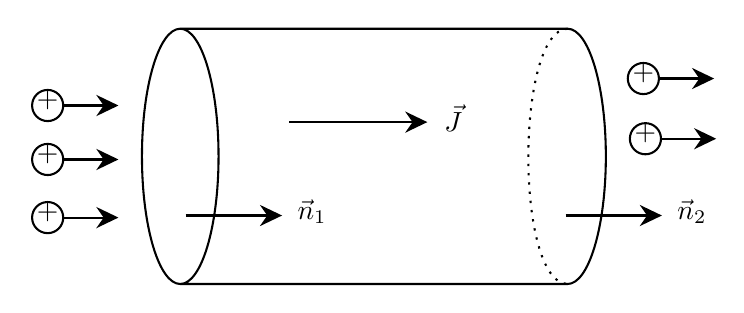
\begin{tikzpicture}[x=0.75pt,y=0.75pt,yscale=-1,xscale=1]
	%uncomment if require: \path (0,300); %set diagram left start at 0, and has height of 300

	%Shape: Can [id:dp017404037796793226] 
	\draw   (113.45,64) -- (300.05,64) .. controls (310.24,64) and (318.5,91.53) .. (318.5,125.5) .. controls (318.5,159.47) and (310.24,187) .. (300.05,187) -- (113.45,187) .. controls (103.26,187) and (95,159.47) .. (95,125.5) .. controls (95,91.53) and (103.26,64) .. (113.45,64) .. controls (123.64,64) and (131.9,91.53) .. (131.9,125.5) .. controls (131.9,159.47) and (123.64,187) .. (113.45,187) ;
	%Curve Lines [id:da8183553062560818] 
	\draw  [dash pattern={on 0.84pt off 2.51pt}]  (300.05,64) .. controls (275.1,64.75) and (274.6,186.25) .. (300.05,187) ;
	%Shape: Circle [id:dp011877859992850626] 
	\draw   (329.07,88) .. controls (329.07,83.86) and (332.42,80.5) .. (336.57,80.5) .. controls (340.71,80.5) and (344.07,83.86) .. (344.07,88) .. controls (344.07,92.14) and (340.71,95.5) .. (336.57,95.5) .. controls (332.42,95.5) and (329.07,92.14) .. (329.07,88) -- cycle ;

	%Straight Lines [id:da44264635934188323] 
	\draw    (344.07,88) -- (367.67,88) ;
	\draw [shift={(370.67,88)}, rotate = 180] [fill={rgb, 255:red, 0; green, 0; blue, 0 }  ][line width=0.08]  [draw opacity=0] (10.72,-5.15) -- (0,0) -- (10.72,5.15) -- (7.12,0) -- cycle    ;
	%Shape: Circle [id:dp2671896177393527] 
	\draw   (330.07,117) .. controls (330.07,112.86) and (333.42,109.5) .. (337.57,109.5) .. controls (341.71,109.5) and (345.07,112.86) .. (345.07,117) .. controls (345.07,121.14) and (341.71,124.5) .. (337.57,124.5) .. controls (333.42,124.5) and (330.07,121.14) .. (330.07,117) -- cycle ;

	%Straight Lines [id:da8934265394022132] 
	\draw    (345.07,117) -- (368.67,117) ;
	\draw [shift={(371.67,117)}, rotate = 180] [fill={rgb, 255:red, 0; green, 0; blue, 0 }  ][line width=0.08]  [draw opacity=0] (10.72,-5.15) -- (0,0) -- (10.72,5.15) -- (7.12,0) -- cycle    ;
	%Shape: Circle [id:dp24014124719456853] 
	\draw   (42.07,101) .. controls (42.07,96.86) and (45.42,93.5) .. (49.57,93.5) .. controls (53.71,93.5) and (57.07,96.86) .. (57.07,101) .. controls (57.07,105.14) and (53.71,108.5) .. (49.57,108.5) .. controls (45.42,108.5) and (42.07,105.14) .. (42.07,101) -- cycle ;

	%Straight Lines [id:da728429653230475] 
	\draw    (57.07,101) -- (80.67,101) ;
	\draw [shift={(83.67,101)}, rotate = 180] [fill={rgb, 255:red, 0; green, 0; blue, 0 }  ][line width=0.08]  [draw opacity=0] (10.72,-5.15) -- (0,0) -- (10.72,5.15) -- (7.12,0) -- cycle    ;
	%Shape: Circle [id:dp707704073297533] 
	\draw   (42.07,127) .. controls (42.07,122.86) and (45.42,119.5) .. (49.57,119.5) .. controls (53.71,119.5) and (57.07,122.86) .. (57.07,127) .. controls (57.07,131.14) and (53.71,134.5) .. (49.57,134.5) .. controls (45.42,134.5) and (42.07,131.14) .. (42.07,127) -- cycle ;

	%Straight Lines [id:da3887493517750147] 
	\draw    (57.07,127) -- (80.67,127) ;
	\draw [shift={(83.67,127)}, rotate = 180] [fill={rgb, 255:red, 0; green, 0; blue, 0 }  ][line width=0.08]  [draw opacity=0] (10.72,-5.15) -- (0,0) -- (10.72,5.15) -- (7.12,0) -- cycle    ;
	%Shape: Circle [id:dp7135595126886061] 
	\draw   (42.07,155) .. controls (42.07,150.86) and (45.42,147.5) .. (49.57,147.5) .. controls (53.71,147.5) and (57.07,150.86) .. (57.07,155) .. controls (57.07,159.14) and (53.71,162.5) .. (49.57,162.5) .. controls (45.42,162.5) and (42.07,159.14) .. (42.07,155) -- cycle ;

	%Straight Lines [id:da6009103508315261] 
	\draw    (57.07,155) -- (80.67,155) ;
	\draw [shift={(83.67,155)}, rotate = 180] [fill={rgb, 255:red, 0; green, 0; blue, 0 }  ][line width=0.08]  [draw opacity=0] (10.72,-5.15) -- (0,0) -- (10.72,5.15) -- (7.12,0) -- cycle    ;
	%Straight Lines [id:da9479029623698474] 
	\draw    (116.07,154) -- (159.5,154) ;
	\draw [shift={(162.5,154)}, rotate = 180] [fill={rgb, 255:red, 0; green, 0; blue, 0 }  ][line width=0.08]  [draw opacity=0] (10.72,-5.15) -- (0,0) -- (10.72,5.15) -- (7.12,0) -- cycle    ;
	%Straight Lines [id:da6793377751043193] 
	\draw    (166.07,109) -- (229.5,109) ;
	\draw [shift={(232.5,109)}, rotate = 180] [fill={rgb, 255:red, 0; green, 0; blue, 0 }  ][line width=0.08]  [draw opacity=0] (10.72,-5.15) -- (0,0) -- (10.72,5.15) -- (7.12,0) -- cycle    ;
	%Straight Lines [id:da8906300638878115] 
	\draw    (299.07,154) -- (342.5,154) ;
	\draw [shift={(345.5,154)}, rotate = 180] [fill={rgb, 255:red, 0; green, 0; blue, 0 }  ][line width=0.08]  [draw opacity=0] (10.72,-5.15) -- (0,0) -- (10.72,5.15) -- (7.12,0) -- cycle    ;

	% Text Node
	\draw (336.57,85.5) node    {$+$};
	% Text Node
	\draw (337.57,114.5) node    {$+$};
	% Text Node
	\draw (49.57,98.5) node    {$+$};
	% Text Node
	\draw (49.57,124.5) node    {$+$};
	% Text Node
	\draw (49.57,152.5) node    {$+$};
	% Text Node
	\draw (177,152) node    {$\vec{n}_{1}$};
	% Text Node
	\draw (245,107) node    {$\vec{J}$};
	% Text Node
	\draw (360,152) node    {$\vec{n}_{2}$};

	\end{tikzpicture}
\end{figure}
\FloatBarrier

Tale equazione sta a significare che se consideriamo un tratto di conduttore in regime stazionario, \emph{tante cariche entrano, tante ne devono uscire}: non ci deve essere accumulo di carica in un conduttore. La superficie laterale del conduttore è allora un tubo di flusso per $\vec{J}$ perché le sue linee devono essere parallele per poter evitare accumulo di carica.

\begin{align*}
	\Phi_{\Sigma}(\vec{J}) &= \int_{\tau}\text{div}\vec{J} d\tau = 0 \\
	&= \underbrace{\int_{\text{sup. lat.}}\vec{J} \cdot \vec{n} dS}_{=0} +\int_{B_2}\vec{J} \cdot \vec{n}_2 dS + \int_{B_1}\vec{J} \cdot (-\vec{n}_1 ) dS \\
	&= \int_{B_2}\vec{J} \cdot \vec{n}_2 dS - \int_{B_1}\vec{J} \cdot \vec{n}_1 dS = 0\\
	&\implies \underbrace{\int_{B_2}\vec{J} \cdot \vec{n}_2 dS}_{I_2} = \underbrace{\int_{B_1}\vec{J} \cdot \vec{n}_1 dS}_{I_1}
\end{align*}

I due integrali rappresentano le correnti che stanno entrando e uscendo dalle basi uno e due. Questa formula ci dice che in regime stazionario la corrente $I_2$ in uscita dal conduttore è pari alla corrente $I_1$ in ingresso.
In condizioni stazionarie l'intensità di corrente è la stessa attraverso ogni sezione del conduttore.

\subsection{Leggi di Kirchhoff}

I circuiti elettrici sono sistemi costituiti dalle interconnessioni di semplici dispositivi detti elementi. Per descrivere il comportamento di tali elementi si utilizzano le variabili tensione e corrente. Gli elementi geometrici distintivi di un circuito sono i nodi e i rami. Un nodo è un punto nel quale convengono almeno tre conduttori. I nodi sono collegati da rami, in cui possono esserci componenti attivi (generatori) o componenti passivi (resistori). All'interno di una rete è possibile individuare determinati cammini chiusi, detti maglie, costituiti da più rami.

Se siamo in regime stazionario, considerando un nodo e chiudendolo in una superficie $\Sigma$, la divergenza di $\vec{J}$ è zero, il flusso di $\vec{J}$ attraverso la superficie chiusa è nullo. Ma, dato che questo flusso di $\vec{J}$ si può interpretare in questo modo:

\[
	\Phi_{\Sigma}(\vec{J} )= 0 = I_1+I_2+I_3 \implies \boxed{\sum_i I_i=0}
\]

considerando positive le correnti uscenti.

Arriviamo a concludere che la sommatoria delle correnti entranti e uscenti da un nodo è zero. Questo risultato è noto come \textbf{prima legge di Kirchhoff}.
Consideriamo ora una maglia del circuito.

\begin{figure}[htpb]
	\centering

	\tikzset{every picture/.style={line width=0.75pt}} %set default line width to 0.75pt        

	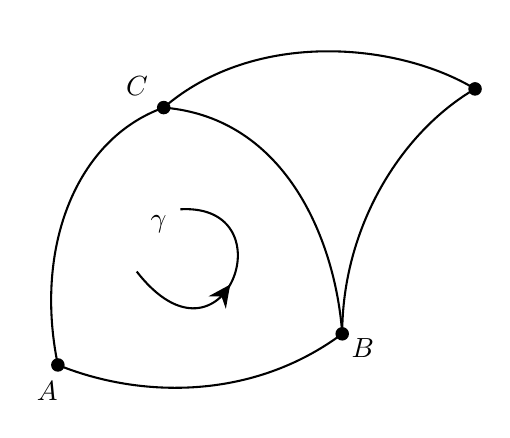
\begin{tikzpicture}[x=0.75pt,y=0.75pt,yscale=-1,xscale=1]
	%uncomment if require: \path (0,300); %set diagram left start at 0, and has height of 300

	%Curve Lines [id:da11127780512440166] 
	\draw    (154.5,66) .. controls (214.5,71) and (237.5,132) .. (240.5,175) ;
	%Curve Lines [id:da10636274290526448] 
	\draw    (154.5,66) .. controls (198.5,28) and (267.62,34.69) .. (304.5,57) ;
	%Curve Lines [id:da8804350288523184] 
	\draw    (240.5,175) .. controls (240.5,124) and (268.5,78) .. (304.5,57) ;
	%Curve Lines [id:da869349992627678] 
	\draw    (103.5,190) .. controls (91.79,133.05) and (112.5,81) .. (154.5,66) ;
	%Curve Lines [id:da43043148147300325] 
	\draw    (240.5,175) .. controls (197.5,207) and (143.42,206.27) .. (103.5,190) ;
	%Curve Lines [id:da40348725078307845] 
	\draw    (141.5,145) .. controls (183.5,199) and (215.5,112) .. (162.5,115) ;
	\draw [shift={(186.54,151.27)}, rotate = 485.9] [fill={rgb, 255:red, 0; green, 0; blue, 0 }  ][line width=0.08]  [draw opacity=0] (10.72,-5.15) -- (0,0) -- (10.72,5.15) -- (7.12,0) -- cycle    ;
	%Shape: Circle [id:dp4401661675359796] 
	\draw  [fill={rgb, 255:red, 0; green, 0; blue, 0 }  ,fill opacity=1 ] (237.75,175) .. controls (237.75,173.48) and (238.98,172.25) .. (240.5,172.25) .. controls (242.02,172.25) and (243.25,173.48) .. (243.25,175) .. controls (243.25,176.52) and (242.02,177.75) .. (240.5,177.75) .. controls (238.98,177.75) and (237.75,176.52) .. (237.75,175) -- cycle ;
	%Shape: Circle [id:dp7453620979054527] 
	\draw  [fill={rgb, 255:red, 0; green, 0; blue, 0 }  ,fill opacity=1 ] (100.75,190) .. controls (100.75,188.48) and (101.98,187.25) .. (103.5,187.25) .. controls (105.02,187.25) and (106.25,188.48) .. (106.25,190) .. controls (106.25,191.52) and (105.02,192.75) .. (103.5,192.75) .. controls (101.98,192.75) and (100.75,191.52) .. (100.75,190) -- cycle ;
	%Shape: Circle [id:dp05292139092767889] 
	\draw  [fill={rgb, 255:red, 0; green, 0; blue, 0 }  ,fill opacity=1 ] (151.75,66) .. controls (151.75,64.48) and (152.98,63.25) .. (154.5,63.25) .. controls (156.02,63.25) and (157.25,64.48) .. (157.25,66) .. controls (157.25,67.52) and (156.02,68.75) .. (154.5,68.75) .. controls (152.98,68.75) and (151.75,67.52) .. (151.75,66) -- cycle ;
	%Shape: Circle [id:dp5530571859485116] 
	\draw  [fill={rgb, 255:red, 0; green, 0; blue, 0 }  ,fill opacity=1 ] (301.75,57) .. controls (301.75,55.48) and (302.98,54.25) .. (304.5,54.25) .. controls (306.02,54.25) and (307.25,55.48) .. (307.25,57) .. controls (307.25,58.52) and (306.02,59.75) .. (304.5,59.75) .. controls (302.98,59.75) and (301.75,58.52) .. (301.75,57) -- cycle ;

	% Text Node
	\draw (152,122) node    {$\gamma $};
	% Text Node
	\draw (98.4,202.8) node    {$A$};
	% Text Node
	\draw (250.4,182) node    {$B$};
	% Text Node
	\draw (141.6,55.6) node    {$C$};

	\end{tikzpicture}
\end{figure}
\FloatBarrier

Ricordando che il campo elettrostatico è conservativo, abbiamo che:

\[
	\oint_{\gamma} \vec{E} \cdot d\vec{l} = 0 = (V_a-V_b  ) + (V_b-V_c  )+ (V_c-V_a  ) = \Delta V_{ab} + \Delta V_{bc} + \Delta V_{ca}
\]

Allora

\[
	\boxed{\sum_i \Delta V_i=0}
\]

Otteniamo così un altro legge, affermante che la sommatoria delle differenze di potenziale calcolate lungo un percorso chiuso deve essere pari a zero. Essa è nota come \textbf{legge di Kirchhoff delle tensioni}.
Queste leggi si applicano a tutti i nodi e a tutte le maglie del circuito. Danno un sistema di equazioni per risolverlo.

\section{Conduttori Ohmici}

Finora abbiamo suddiviso i materiali tra isolanti e conduttori perfetti, ma in realtà la suddivisione non è così netta. Ci sono materiali che a seconda delle situazioni possono comportarsi o da isolanti o da conduttori. Gli isolanti non perfetti ad esempio presentano proprietà conduttrici. Si parla di conduttori ohmici perché fu Ohm a studiarne le proprietà conduttive. Egli scoprì che in regime stazionario, la d.d.p. applicata ai capi di un conduttore metallico e l'intensità di corrente che a seguito di ciò lo attraversa, è pari ad una grandezza, detta resistenza del conduttore, che dipende solamente dal conduttore e dalle sue dimensioni. Quindi i conduttori ohmici sono quei conduttori la cui qualità di opporsi al transito di una corrente di cariche è misurata dalla seguente legge.

\[
	\boxed{\Delta V= RI} \qquad \text{legge di Ohm}
\]

Per i conduttori a sezione costante, la resistenza $ R $ del conduttore ha la seguente forma

\[
	R = \rho \frac{l}{S} = \frac{1}{\sigma}\frac{l}{S}
\]

Dove $ \rho $ è la resistività del materiale conduttore.
Inoltre $ \frac{1}{\rho}= \sigma $ è detta conducibilità (o conduttività).

\begin{figure}[htpb]
	\centering

	\tikzset{every picture/.style={line width=0.75pt}} %set default line width to 0.75pt        

	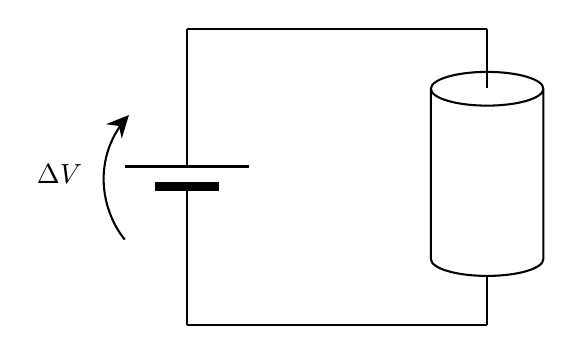
\begin{tikzpicture}[x=0.75pt,y=0.75pt,yscale=-1,xscale=1]
	%uncomment if require: \path (0,300); %set diagram left start at 0, and has height of 300

	%Shape: Battery [id:dp6291306635732892] 
	\draw  [fill={rgb, 255:red, 0; green, 0; blue, 0 }  ,fill opacity=1 ] (168.3,180.8) -- (168.3,144.8) (138.3,136.8) -- (198.3,136.8) (168.3,136.8) -- (168.3,100.8) (153.3,148) -- (153.3,144.8) -- (183.3,144.8) -- (183.3,148) -- (153.3,148) -- cycle ;
	%Straight Lines [id:da46883367559070654] 
	\draw    (168.3,70.4) -- (312.8,70.4) ;
	%Straight Lines [id:da743496792064678] 
	\draw    (312.8,99.2) -- (312.8,70.4) ;
	%Straight Lines [id:da1990389962662249] 
	\draw    (312.8,213.2) -- (312.8,189.4) ;
	%Straight Lines [id:da11413330658688636] 
	\draw    (168.3,213.2) -- (312.8,213.2) ;
	%Straight Lines [id:da38694099187961495] 
	\draw    (168.3,213.2) -- (168.3,180.8) ;
	%Curve Lines [id:da2620092915211867] 
	\draw    (138.2,172) .. controls (126.43,157.33) and (122.85,132.98) .. (138.43,114.04) ;
	\draw [shift={(140.2,112)}, rotate = 492.51] [fill={rgb, 255:red, 0; green, 0; blue, 0 }  ][line width=0.08]  [draw opacity=0] (10.72,-5.15) -- (0,0) -- (10.72,5.15) -- (7.12,0) -- cycle    ;
	%Shape: Can [id:dp7370813713893971] 
	\draw   (339.9,99.33) -- (339.9,181.37) .. controls (339.9,185.86) and (327.77,189.5) .. (312.8,189.5) .. controls (297.83,189.5) and (285.7,185.86) .. (285.7,181.37) -- (285.7,99.33) .. controls (285.7,94.84) and (297.83,91.2) .. (312.8,91.2) .. controls (327.77,91.2) and (339.9,94.84) .. (339.9,99.33) .. controls (339.9,103.82) and (327.77,107.46) .. (312.8,107.46) .. controls (297.83,107.46) and (285.7,103.82) .. (285.7,99.33) ;
	%Straight Lines [id:da5695340545261522] 
	\draw    (168.3,100.8) -- (168.3,70.4) ;

	% Text Node
	\draw (106.8,140.6) node    {$\Delta V$};

	\end{tikzpicture}
\end{figure}
\FloatBarrier

Dalla legge di Ohm deriva che le dimensioni della resistenza sono quelle di una differenza di potenziale divisa una corrente. Vista l'importanza della grandezza, ribattezziamo questa unità di misura come $\Omega$. Invece di ragionare in termini di resistenza, si può ragionare in termini di inverso di resistenza: $ G=1/R $. Tale grandezza viene chiamata \textbf{conduttanza}. La sua unità di misura sarebbe $\Omega^{-1}$, anche se viene ribattezzata \emph{Siemens} (o anche \emph{mho}).

\begin{figure}[htpb]
	\centering

	\tikzset{every picture/.style={line width=0.75pt}} %set default line width to 0.75pt        

	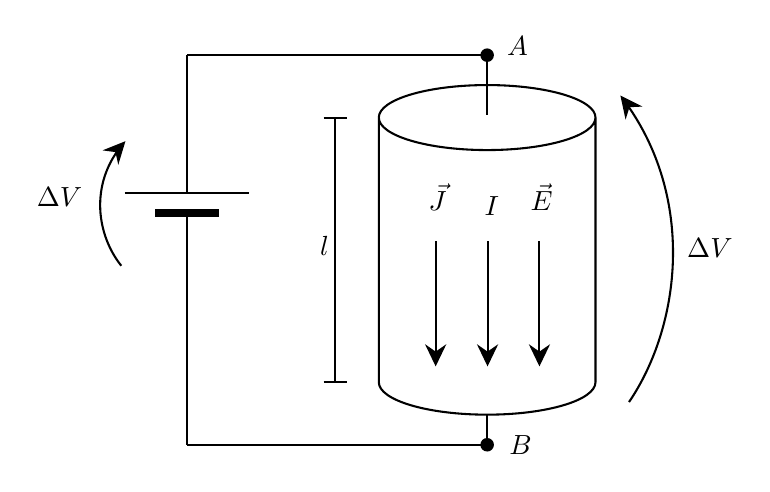
\begin{tikzpicture}[x=0.75pt,y=0.75pt,yscale=-1,xscale=1]
	%uncomment if require: \path (0,300); %set diagram left start at 0, and has height of 300

	%Shape: Battery [id:dp22509077003774736] 
	\draw  [fill={rgb, 255:red, 0; green, 0; blue, 0 }  ,fill opacity=1 ] (188.3,171.95) -- (188.3,135.95) (158.3,127.95) -- (218.3,127.95) (188.3,127.95) -- (188.3,91.95) (173.3,139.15) -- (173.3,135.95) -- (203.3,135.95) -- (203.3,139.15) -- (173.3,139.15) -- cycle ;
	%Straight Lines [id:da7219445667701057] 
	\draw    (188.3,61.55) -- (332.8,61.55) ;
	%Straight Lines [id:da19489332319438146] 
	\draw    (332.8,90.35) -- (332.8,61.55) ;
	%Straight Lines [id:da7739814888159238] 
	\draw    (332.8,249.25) -- (332.8,234.75) ;
	%Straight Lines [id:da34455176440645685] 
	\draw    (188.3,249.25) -- (332.8,249.25) ;
	%Straight Lines [id:da19332381310739422] 
	\draw    (188.3,249.25) -- (188.3,171.95) ;
	%Curve Lines [id:da7997142849254137] 
	\draw    (156.53,163) .. controls (144.76,148.33) and (141.18,123.98) .. (156.76,105.04) ;
	\draw [shift={(158.53,103)}, rotate = 492.51] [fill={rgb, 255:red, 0; green, 0; blue, 0 }  ][line width=0.08]  [draw opacity=0] (10.72,-5.15) -- (0,0) -- (10.72,5.15) -- (7.12,0) -- cycle    ;
	%Shape: Can [id:dp14099858415964261] 
	\draw   (385,91.61) -- (385,219.09) .. controls (385,227.74) and (361.63,234.75) .. (332.8,234.75) .. controls (303.97,234.75) and (280.6,227.74) .. (280.6,219.09) -- (280.6,91.61) .. controls (280.6,82.96) and (303.97,75.95) .. (332.8,75.95) .. controls (361.63,75.95) and (385,82.96) .. (385,91.61) .. controls (385,100.26) and (361.63,107.27) .. (332.8,107.27) .. controls (303.97,107.27) and (280.6,100.26) .. (280.6,91.61) ;
	%Straight Lines [id:da26449592927404764] 
	\draw    (188.3,91.95) -- (188.3,61.55) ;
	%Straight Lines [id:da7576221257386357] 
	\draw    (308,151.25) -- (308,208.5) ;
	\draw [shift={(308,211.5)}, rotate = 270] [fill={rgb, 255:red, 0; green, 0; blue, 0 }  ][line width=0.08]  [draw opacity=0] (10.72,-5.15) -- (0,0) -- (10.72,5.15) -- (7.12,0) -- cycle    ;
	%Shape: Circle [id:dp6264100912992732] 
	\draw  [fill={rgb, 255:red, 0; green, 0; blue, 0 }  ,fill opacity=1 ] (330.05,61.55) .. controls (330.05,60.03) and (331.28,58.8) .. (332.8,58.8) .. controls (334.32,58.8) and (335.55,60.03) .. (335.55,61.55) .. controls (335.55,63.07) and (334.32,64.3) .. (332.8,64.3) .. controls (331.28,64.3) and (330.05,63.07) .. (330.05,61.55) -- cycle ;
	%Straight Lines [id:da13078567924346718] 
	\draw    (333,151.25) -- (333,208.5) ;
	\draw [shift={(333,211.5)}, rotate = 270] [fill={rgb, 255:red, 0; green, 0; blue, 0 }  ][line width=0.08]  [draw opacity=0] (10.72,-5.15) -- (0,0) -- (10.72,5.15) -- (7.12,0) -- cycle    ;
	%Straight Lines [id:da8093452580702538] 
	\draw    (358,151.25) -- (358,208.5) ;
	\draw [shift={(358,211.5)}, rotate = 270] [fill={rgb, 255:red, 0; green, 0; blue, 0 }  ][line width=0.08]  [draw opacity=0] (10.72,-5.15) -- (0,0) -- (10.72,5.15) -- (7.12,0) -- cycle    ;
	%Shape: Circle [id:dp24588222328028175] 
	\draw  [fill={rgb, 255:red, 0; green, 0; blue, 0 }  ,fill opacity=1 ] (330.05,249.25) .. controls (330.05,247.73) and (331.28,246.5) .. (332.8,246.5) .. controls (334.32,246.5) and (335.55,247.73) .. (335.55,249.25) .. controls (335.55,250.77) and (334.32,252) .. (332.8,252) .. controls (331.28,252) and (330.05,250.77) .. (330.05,249.25) -- cycle ;
	%Shape: Boxed Bezier Curve [id:dp0474784471536458] 
	\draw    (401.16,228.67) .. controls (426.17,191.82) and (433.41,130.14) .. (398.62,83.14) ;
	\draw [shift={(397,81)}, rotate = 412.22] [fill={rgb, 255:red, 0; green, 0; blue, 0 }  ][line width=0.08]  [draw opacity=0] (10.72,-5.15) -- (0,0) -- (10.72,5.15) -- (7.12,0) -- cycle    ;
	%Straight Lines [id:da7317171609485253] 
	\draw    (259.6,219.09) -- (259.6,91.61) ;
	\draw [shift={(259.6,91.61)}, rotate = 450] [color={rgb, 255:red, 0; green, 0; blue, 0 }  ][line width=0.75]    (0,5.59) -- (0,-5.59)   ;
	\draw [shift={(259.6,219.09)}, rotate = 450] [color={rgb, 255:red, 0; green, 0; blue, 0 }  ][line width=0.75]    (0,5.59) -- (0,-5.59)   ;

	% Text Node
	\draw (126.8,129.93) node    {$\Delta V$};
	% Text Node
	\draw (309,130) node    {$\vec{J}$};
	% Text Node
	\draw (347.4,57.3) node    {$A$};
	% Text Node
	\draw (335,134) node    {$I$};
	% Text Node
	\draw (359,130) node    {$\vec{E}$};
	% Text Node
	\draw (348.9,249.3) node    {$B$};
	% Text Node
	\draw (440.13,154.6) node    {$\Delta V$};
	% Text Node
	\draw (254.4,153.3) node    {$l$};

	\end{tikzpicture}
\end{figure}
\FloatBarrier

Consideriamo ora un regime di conduzione stazionaria e un conduttore omogeneo:

\begin{equation}
	\begin{aligned}
		\Delta V &= \int_A^B \vec{E} \cdot d\vec{l} = El \\
		RI       &=El \\
		\rho \frac{l}{S} \cdot I &= El \\
		\rho \frac{l}{S} \cdot JS &= El \\
		\rho J &= E \implies \boxed{\vec{E} = \rho \vec{J}} \qquad \text{oppure} \qquad \boxed{\vec{J} = \sigma\vec{E}}
	\end{aligned}
\end{equation}

Le ultime due relazioni sono note come legge di Ohm in forma locale.

Per un conduttore non-ohmico, si ha $ \vec{J} = f(\vec{E} ) $ ossia i due vettori non sono in relazione lineare tra loro.

Nel caso di conduttori non isotropi, introducendo $ \sigma $ come tensore conducibilità si ha $J_i= \Sigma_k\sigma_{ik}E_k$.

\section{Modello di Drude-Lorentz della conduzione}

Agli inizi nel 900 fu introdotto un modello microscopico che spiega il legame fra $J$ ed $E$ in base alla dinamica microscopica dei portatori di carica. Tale modello fu proposto da Drude e successivamente sviluppato da Lorentz. Si suppone che gli ioni del reticolo cristallino siano fissi e che gli elettroni si muovano attraverso il reticolo in modo completamente disordinato.

\begin{figure}[htpb]
	\centering

	\tikzset{every picture/.style={line width=0.75pt}} %set default line width to 0.75pt        

	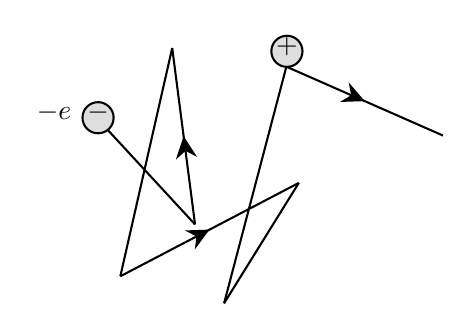
\begin{tikzpicture}[x=0.75pt,y=0.75pt,yscale=-1,xscale=1]
	%uncomment if require: \path (0,300); %set diagram left start at 0, and has height of 300

	%Shape: Circle [id:dp6561318663921207] 
	\draw  [fill={rgb, 255:red, 222; green, 222; blue, 222 }  ,fill opacity=1 ] (226.27,82.6) .. controls (226.27,78.46) and (229.62,75.1) .. (233.77,75.1) .. controls (237.91,75.1) and (241.27,78.46) .. (241.27,82.6) .. controls (241.27,86.74) and (237.91,90.1) .. (233.77,90.1) .. controls (229.62,90.1) and (226.27,86.74) .. (226.27,82.6) -- cycle ;

	%Straight Lines [id:da4580037288020633] 
	\draw    (147,120) -- (189.5,166) ;
	%Straight Lines [id:da29394536279820804] 
	\draw    (189.5,166) -- (178.5,81) ;
	\draw [shift={(184,123.5)}, rotate = 442.63] [fill={rgb, 255:red, 0; green, 0; blue, 0 }  ][line width=0.08]  [draw opacity=0] (10.72,-5.15) -- (0,0) -- (10.72,5.15) -- (7.12,0) -- cycle    ;
	%Straight Lines [id:da3085778409379849] 
	\draw    (178.5,81) -- (153.5,191) ;
	%Straight Lines [id:da30789847434685935] 
	\draw    (153.5,191) -- (239.5,146) ;
	\draw [shift={(196.5,168.5)}, rotate = 512.38] [fill={rgb, 255:red, 0; green, 0; blue, 0 }  ][line width=0.08]  [draw opacity=0] (10.72,-5.15) -- (0,0) -- (10.72,5.15) -- (7.12,0) -- cycle    ;
	%Straight Lines [id:da31112340431688956] 
	\draw    (239.5,146) -- (203.5,204) ;
	%Straight Lines [id:da6816397380460644] 
	\draw    (203.5,204) -- (233.5,90) ;
	%Straight Lines [id:da14431912970181138] 
	\draw    (309,123.2) -- (233.5,90) ;
	\draw [shift={(271.25,106.6)}, rotate = 203.74] [fill={rgb, 255:red, 0; green, 0; blue, 0 }  ][line width=0.08]  [draw opacity=0] (10.72,-5.15) -- (0,0) -- (10.72,5.15) -- (7.12,0) -- cycle    ;
	%Shape: Circle [id:dp922295589505471] 
	\draw  [fill={rgb, 255:red, 222; green, 222; blue, 222 }  ,fill opacity=1 ] (135.27,114.6) .. controls (135.27,110.46) and (138.62,107.1) .. (142.77,107.1) .. controls (146.91,107.1) and (150.27,110.46) .. (150.27,114.6) .. controls (150.27,118.74) and (146.91,122.1) .. (142.77,122.1) .. controls (138.62,122.1) and (135.27,118.74) .. (135.27,114.6) -- cycle ;

	% Text Node
	\draw (233.77,80.1) node    {$+$};
	% Text Node
	\draw (142.77,112.1) node    {$-$};
	% Text Node
	\draw (121.6,112) node    {$-e$};

	\end{tikzpicture}
\end{figure}
\FloatBarrier

Nel loro moto gli elettroni subiscono continue interazioni con gli ioni, che chiamiamo urti: tra un urto e il successivo il moto è libero e la traiettoria rettilinea, cosicché la traiettoria di ciascun elettrone è costituita da una successione di segmenti rettilinei, con direzione e lunghezza variabili. L'insieme delle traiettorie è completamente casuale e non si ha un flusso di carica netto, cioè una corrente, in nessuna direzione. Il modello di D-L suppone che la velocità con cui un elettrone emerge dall'urto sia completamente casuale. Si introducono due quantità:

\begin{itemize}
	\item libero cammino medio del portatore di carica, $l$: è la distanza media che un elettrone percorre fra due urti. Si tratta di un processo molto casuale, ecco perché parliamo di una quantità media.
	\item Tempo medio fra due urti, $\tau$. Tale tempo è legato al cammino medio perché se conosciamo la velocità quadratica media, possiamo legare le due quantità come
	\[
		\tau = \frac{l}{\overline{v}}
	\]
\end{itemize}

La velocità quadratica media dipende dalla temperatura del materiale. Si può dimostrare che:

\[
	\frac{1}{2} m_e \overline{v}^2 = \frac{3}{2} kT
\]

Quando si applica un campo elettrico $E$ ciascun elettrone acquista Un'accelerazione $a=\frac{F}{m}=\frac{-eE}{m}$ opposta al campo elettrico, e i tratti rettilinei tra due urti diventano archi di parabola. Alla distribuzione casuale e isotropa della velocità si sovrappone una velocità $ v_d  $ di deriva. Essendo questa velocità piccola rispetto a quella propria degli elettroni, il tempo medio $ \tau  $ fra due urti non cambia.

\[
	\vec{F} = -e\vec{E} \qquad \vec{a} =\frac{\vec{F}}{m_e} = - \frac{e\vec{E}}{m_e}
\]

Supponiamo che l'elettrone $i$-esimo abbia subito un urto e che ne esca con una certa velocità che chiameremo $v_i^{(-)}$, completamente scorrelata da quella passata. Se indichiamo con $v_i^{(+)}$ la velocità dell'elettrone subito prima dell'urto successivo, abbiamo:

\begin{gather*}
	\vec{v}_i^{(+)}(t) = \vec{v}_i^{(-)} + \vec{a}t = \vec{v}_i^{(-)} - \frac{e\vec{E}}{m_e} t \\
	\vec{v}_i^{(+)}(\tau_i) = \vec{v}_i^{(-)} - \frac{e\vec{E}}{m_e} \tau_i
\end{gather*}

Facendo la media su un grande numero di urti possiamo definire la velocità di deriva come:

\[
	\langle \vec{v}_i^{(+)} (\tau_i) \rangle = \vec{v}_d \qquad \langle \vec{v}_i^{(+)}(\tau_i) \rangle = \langle \vec{v}_i^{(-)} \rangle - \frac{e\vec{E}}{m_e} \langle \tau_i \rangle
\]

La media non cambia il termine contenente il campo elettrico, che è uguale per tutti gli elettroni. Inoltre la $ \langle \vec{v}_i^{(-)} \rangle = 0 $ in quanto dopo ogni urto la distribuzione delle velocità rimane casuale. Pertanto:

\[
	\vec{v}_d  = \underbrace{\langle \vec{v}_i^{(-)} \rangle}_{=0} - \frac{e\vec{E}}{m_e} \underbrace{\langle \tau_i \rangle}_{=\tau} = - \frac{e\vec{E}}{m_e} \tau
\]

Per effetto del campo elettrico $E$ ciascun elettrone nel metallo acquista una velocità $ v_d  $ nella direzione del campo elettrico, che è proporzionale al campo elettrico stesso. In sostanza si ammette che in media l'urto cancelli la direzione preferenziale del moto dovuta all'azione del campo elettrico e che questa venga ristabilita durante il tempo $\tau$. La densità di corrente elettrica che consegue a questo moto ordinato è:

\[
	\vec{J} =nq\vec{v}_d \implies J = n(-e)\left( -\frac{e\vec{E}\tau}{m_e} \right) = \underbrace{\left( \frac{ne^2 \tau}{m_e} \right)}_{\sigma}  \vec{E}
\]

Ritorna il risultato $ \vec{J} = \sigma \vec{E}  $ con $ \sigma = \frac{ne^2 \tau}{m_e} $.
Per avere elevata conducibilità è necessario avere un gran numero di portatori di carica e un tempo medio fra i due urti molto grande, perché questi disturbano il processo di conduzione. Al limite, in un super conduttore, $\tau$ tende ad infinito.
Se aumentiamo la temperatura, aumenta la velocità quadratica media e quindi l'intervallo di tempo fra due urti diminuisce e diminuisce la conduttività. La relazione trovata è nota come legge di Ohm della conduzione elettrica e stabilisce che il rapporto tra la densità di corrente $J$ e il campo elettrico applicato $\vec{E}$ è dato da una grandezza caratteristica del conduttore. Il fatto che la conduttività sia sempre positiva, ribadisce il fatto che la densità di corrente è concorde al campo elettrico indipendentemente dal segno dei portatori di carica.

\subsection{Conduttore ohmico di forma generica}

Abbiamo visto che nel caso di un conduttore di sezione regolare si ha: $ R = \frac{l}{S}\rho $.
Non sempre abbiamo conduttori dotati di una forma tale per cui la sezione è regolare. Stiamo considerando conduttori ohmici, per cui la legge di Ohm continua a valere, il problema è trovarne la resistenza. In tal caso possiamo immaginare di suddividere il conduttore in tante fettine sottili di spessore $dl$ e sezione $S$, che dipenderà dalla posizione.

\begin{figure}[htpb]
	\centering

	% Pattern Info
	 
	\tikzset{
	pattern size/.store in=\mcSize, 
	pattern size = 5pt,
	pattern thickness/.store in=\mcThickness, 
	pattern thickness = 0.3pt,
	pattern radius/.store in=\mcRadius, 
	pattern radius = 1pt}
	\makeatletter
	\pgfutil@ifundefined{pgf@pattern@name@_y3lhcvofb}{
	\pgfdeclarepatternformonly[\mcThickness,\mcSize]{_y3lhcvofb}
	{\pgfqpoint{0pt}{0pt}}
	{\pgfpoint{\mcSize+\mcThickness}{\mcSize+\mcThickness}}
	{\pgfpoint{\mcSize}{\mcSize}}
	{
	\pgfsetcolor{\tikz@pattern@color}
	\pgfsetlinewidth{\mcThickness}
	\pgfpathmoveto{\pgfqpoint{0pt}{0pt}}
	\pgfpathlineto{\pgfpoint{\mcSize+\mcThickness}{\mcSize+\mcThickness}}
	\pgfusepath{stroke}
	}}
	\makeatother
	\tikzset{every picture/.style={line width=0.75pt}} %set default line width to 0.75pt        

	\begin{tikzpicture}[x=0.75pt,y=0.75pt,yscale=-1,xscale=1]
	%uncomment if require: \path (0,300); %set diagram left start at 0, and has height of 300

	%Shape: Ellipse [id:dp6484887179203112] 
	\draw   (104,145) .. controls (104,100.82) and (114.86,65) .. (128.25,65) .. controls (141.64,65) and (152.5,100.82) .. (152.5,145) .. controls (152.5,189.18) and (141.64,225) .. (128.25,225) .. controls (114.86,225) and (104,189.18) .. (104,145) -- cycle ;
	%Curve Lines [id:da8157123722318489] 
	\draw    (128.25,65) .. controls (195.5,65) and (225.5,163) .. (335.5,110) ;
	%Curve Lines [id:da5839389048384083] 
	\draw    (128.25,225) .. controls (195.5,225) and (225.5,130.3) .. (335.5,181.51) ;
	%Shape: Ellipse [id:dp8581699542787002] 
	\draw  [pattern=_y3lhcvofb,pattern size=6pt,pattern thickness=0.75pt,pattern radius=0pt, pattern color={rgb, 255:red, 222; green, 222; blue, 222}] (208.4,146) .. controls (208.4,126.23) and (213.26,110.2) .. (219.25,110.2) .. controls (225.24,110.2) and (230.1,126.23) .. (230.1,146) .. controls (230.1,165.77) and (225.24,181.8) .. (219.25,181.8) .. controls (213.26,181.8) and (208.4,165.77) .. (208.4,146) -- cycle ;
	%Curve Lines [id:da06702468969463737] 
	\draw    (335.5,110) .. controls (349.4,110) and (349.4,180.8) .. (335.5,181.51) ;
	%Curve Lines [id:da7199387975350722] 
	\draw  [dash pattern={on 0.84pt off 2.51pt}]  (335.5,181.51) .. controls (323.8,181.6) and (323,110.8) .. (335.5,110) ;
	%Curve Lines [id:da3014728401967599] 
	\draw    (211.87,198.2) .. controls (219.44,191.99) and (231.42,185.96) .. (242.68,181.78) ;
	\draw [shift={(245.4,180.8)}, rotate = 520.79] [fill={rgb, 255:red, 0; green, 0; blue, 0 }  ][line width=0.08]  [draw opacity=0] (10.72,-5.15) -- (0,0) -- (10.72,5.15) -- (7.12,0) -- cycle    ;
	\draw [shift={(209.6,200.2)}, rotate = 316.51] [fill={rgb, 255:red, 0; green, 0; blue, 0 }  ][line width=0.08]  [draw opacity=0] (10.72,-5.15) -- (0,0) -- (10.72,5.15) -- (7.12,0) -- cycle    ;
	%Curve Lines [id:da1333721569231685] 
	\draw    (138.98,256.95) .. controls (198.67,275.37) and (288.44,265.66) .. (346.85,210.06) ;
	\draw [shift={(135.36,255.78)}, rotate = 18.51] [fill={rgb, 255:red, 0; green, 0; blue, 0 }  ][line width=0.08]  [draw opacity=0] (10.72,-5.15) -- (0,0) -- (10.72,5.15) -- (7.12,0) -- cycle    ;
	%Straight Lines [id:da5495637004127791] 
	\draw    (47.5,145) -- (125.25,145) ;
	\draw [shift={(128.25,145)}, rotate = 180] [fill={rgb, 255:red, 0; green, 0; blue, 0 }  ][line width=0.08]  [draw opacity=0] (10.72,-5.15) -- (0,0) -- (10.72,5.15) -- (7.12,0) -- cycle    ;

	% Text Node
	\draw (230.4,202.7) node    {$dl$};
	% Text Node
	\draw (126.8,237.5) node    {$A$};
	% Text Node
	\draw (336,192.7) node    {$B$};
	% Text Node
	\draw (307.13,252.6) node    {$\Delta V$};
	% Text Node
	\draw (61.4,131.7) node    {$I$};
	% Text Node
	\draw (251.4,145.7) node    {$S( P)$};

	\end{tikzpicture}
\end{figure}
\FloatBarrier

Supporremo che la conduzione avvenga in regime stazionario, e che quindi la corrente sia la stessa attraverso qualsiasi sezione del conduttore.

\begin{align*}
	\Delta V &= \int_A^B \vec{E} \cdot d\vec{l} =\int_A^B \rho \vec{J} \cdot d\vec{l} =  \\
	&= \int_A^B \rho Jdl = \int_A^B \rho \frac{I}{S}dl= \\
	&= I \underbrace{\int_A^B \frac{\rho dl}{S}}_R = I \cdot R
\end{align*}

Allora

\[
	\boxed{R = \int_A^B \frac{\rho dl}{S}}
\]

\section{Resistori in serie o in parallelo}

Conduttori ohmici caratterizzati da un determinato valore della resistenza sono elementi molto usati nei circuiti elettrici: essi vengono chiamati resistori. Più resistori possono essere collegati tra loro, tipicamente da fili o piattine metallici, la cui resistenza è di norma completamente trascurabile. I collegamenti di base, similmente a quanto già visto per i condensatori, sono in serie e in parallelo.

\subsection{Resistori in serie}

Due resistori sono collegati in serie quando hanno un estremo in comune: in regime stazionario l'intensità di corrente che li attraversa è la stessa.

\begin{figure}[htpb]
	\centering

	\tikzset{every picture/.style={line width=0.75pt}} %set default line width to 0.75pt        

	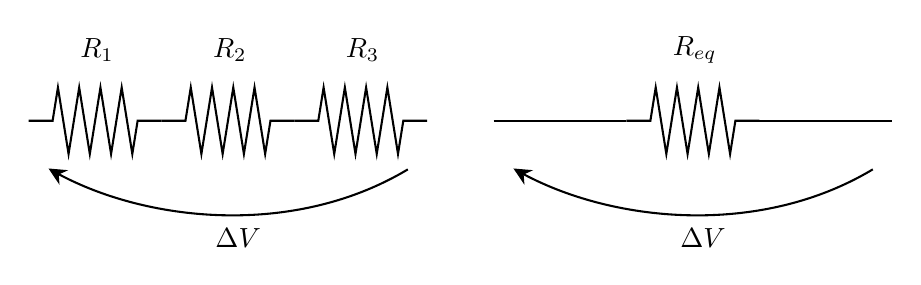
\begin{tikzpicture}[x=0.75pt,y=0.75pt,yscale=-0.8,xscale=0.8]
	%uncomment if require: \path (0,300); %set diagram left start at 0, and has height of 300

	%Shape: Resistor [id:dp7046608827348249] 
	\draw   (59,103) -- (73.4,103) -- (76.6,83) -- (83,123) -- (89.4,83) -- (95.8,123) -- (102.2,83) -- (108.6,123) -- (115,83) -- (121.4,123) -- (124.6,103) -- (139,103) ;
	%Straight Lines [id:da221312075114799] 
	\draw    (339,103) -- (419,103) ;
	%Shape: Resistor [id:dp4547309195494975] 
	\draw   (139,103) -- (153.4,103) -- (156.6,83) -- (163,123) -- (169.4,83) -- (175.8,123) -- (182.2,83) -- (188.6,123) -- (195,83) -- (201.4,123) -- (204.6,103) -- (219,103) ;
	%Shape: Resistor [id:dp5319707454231064] 
	\draw   (219,103) -- (233.4,103) -- (236.6,83) -- (243,123) -- (249.4,83) -- (255.8,123) -- (262.2,83) -- (268.6,123) -- (275,83) -- (281.4,123) -- (284.6,103) -- (299,103) ;
	%Curve Lines [id:da4202906418080372] 
	\draw    (74.24,133.66) .. controls (128.61,164.09) and (218.39,173.69) .. (287.33,132.3) ;
	\draw [shift={(70.95,131.77)}, rotate = 30.58] [fill={rgb, 255:red, 0; green, 0; blue, 0 }  ][line width=0.08]  [draw opacity=0] (10.72,-5.15) -- (0,0) -- (10.72,5.15) -- (7.12,0) -- cycle    ;
	%Shape: Resistor [id:dp10924022597816418] 
	\draw   (419,103) -- (433.4,103) -- (436.6,83) -- (443,123) -- (449.4,83) -- (455.8,123) -- (462.2,83) -- (468.6,123) -- (475,83) -- (481.4,123) -- (484.6,103) -- (499,103) ;
	%Curve Lines [id:da3418165600857359] 
	\draw    (354.24,133.66) .. controls (408.61,164.09) and (498.39,173.69) .. (567.33,132.3) ;
	\draw [shift={(350.95,131.77)}, rotate = 30.58] [fill={rgb, 255:red, 0; green, 0; blue, 0 }  ][line width=0.08]  [draw opacity=0] (10.72,-5.15) -- (0,0) -- (10.72,5.15) -- (7.12,0) -- cycle    ;
	%Straight Lines [id:da6514510472385655] 
	\draw    (499,103) -- (579,103) ;

	% Text Node
	\draw (185.13,173.6) node    {$\Delta V$};
	% Text Node
	\draw (465.13,173.6) node    {$\Delta V$};
	% Text Node
	\draw (100.13,60.6) node    {$R_{1}$};
	% Text Node
	\draw (180.13,60.6) node    {$R_{2}$};
	% Text Node
	\draw (260.13,60.6) node    {$R_{3}$};
	% Text Node
	\draw (460.13,60.6) node    {$R_{eq}$};

	\end{tikzpicture}
\end{figure}
\FloatBarrier

Applicando la legge di Ohm ai resistori si dimostra che $N$ resistori in serie si comportano come un unico resistore di resistenza equivalente:

\[
	\boxed{R_{eq} = \sum_i^N R_i}
\]

\subsection{Resistori in parallelo}

Due resistori si dicono in parallelo quando sono collegati tra loro entrambi gli estremi. In questo caso l'elemento in comune fra i resistori è la differenza di potenziale e quindi, in base alla legge di Ohm, essi sono attraversati da due correnti diverse se i valori delle resistenze sono diverse. Si può dimostrare che $N$ resistori in parallelo si comportano come un unico resistore equivalente di resistenza tale per cui

\[
	\boxed{\frac{1}{R_{eq}} = \sum_i^N \frac{1}{R_i}}
\]

\section{Proprietà generali dei conduttori ohmici in regime stazionario}

Nel caso di conduttori non perfetti, che presentano quindi delle molecole polarizzabili, oltre alla resistività, possiamo attribuire al conduttore anche una costante dielettrica relativa. Avremo allora:

\begin{gather*}
	\text{div}\vec{J} = 0 \qquad \frac{\partial \rho_l}{\partial t} =0\\
	\vec{J} = \sigma \vec{E} \qquad \vec{E} = \rho \vec{J} \qquad \text{div}(\rho \vec{J} ) = \frac{\rho_l}{\varepsilon}
\end{gather*}

Consideriamo due conduttori in serie collegati come in figura, con resistività differenti.

\begin{figure}[htpb]
	\centering

	% Pattern Info
	 
	\tikzset{
	pattern size/.store in=\mcSize, 
	pattern size = 5pt,
	pattern thickness/.store in=\mcThickness, 
	pattern thickness = 0.3pt,
	pattern radius/.store in=\mcRadius, 
	pattern radius = 1pt}
	\makeatletter
	\pgfutil@ifundefined{pgf@pattern@name@_94gxm1s4l}{
	\pgfdeclarepatternformonly[\mcThickness,\mcSize]{_94gxm1s4l}
	{\pgfqpoint{0pt}{0pt}}
	{\pgfpoint{\mcSize+\mcThickness}{\mcSize+\mcThickness}}
	{\pgfpoint{\mcSize}{\mcSize}}
	{
	\pgfsetcolor{\tikz@pattern@color}
	\pgfsetlinewidth{\mcThickness}
	\pgfpathmoveto{\pgfqpoint{0pt}{0pt}}
	\pgfpathlineto{\pgfpoint{\mcSize+\mcThickness}{\mcSize+\mcThickness}}
	\pgfusepath{stroke}
	}}
	\makeatother
	\tikzset{every picture/.style={line width=0.75pt}} %set default line width to 0.75pt        

	\begin{tikzpicture}[x=0.75pt,y=0.75pt,yscale=-0.9,xscale=0.9]
	%uncomment if require: \path (0,300); %set diagram left start at 0, and has height of 300

	%Straight Lines [id:da5492661277472597] 
	\draw    (36.33,145.5) -- (111.22,145.5) ;
	\draw [shift={(114.22,145.5)}, rotate = 180] [fill={rgb, 255:red, 0; green, 0; blue, 0 }  ][line width=0.08]  [draw opacity=0] (10.72,-5.15) -- (0,0) -- (10.72,5.15) -- (7.12,0) -- cycle    ;
	%Straight Lines [id:da3932330408325475] 
	\draw    (180.07,140) -- (243.5,140) ;
	\draw [shift={(246.5,140)}, rotate = 180] [fill={rgb, 255:red, 0; green, 0; blue, 0 }  ][line width=0.08]  [draw opacity=0] (10.72,-5.15) -- (0,0) -- (10.72,5.15) -- (7.12,0) -- cycle    ;
	%Shape: Can [id:dp33923703592669496] 
	\draw   (109.45,84) -- (507.05,84) .. controls (517.24,84) and (525.5,111.53) .. (525.5,145.5) .. controls (525.5,179.47) and (517.24,207) .. (507.05,207) -- (109.45,207) .. controls (99.26,207) and (91,179.47) .. (91,145.5) .. controls (91,111.53) and (99.26,84) .. (109.45,84) .. controls (119.64,84) and (127.9,111.53) .. (127.9,145.5) .. controls (127.9,179.47) and (119.64,207) .. (109.45,207) ;
	%Curve Lines [id:da0015840017294836972] 
	\draw  [dash pattern={on 0.84pt off 2.51pt}]  (510.05,84) .. controls (485.1,84.75) and (484.6,206.25) .. (510.05,207) ;
	%Shape: Ellipse [id:dp9413302304121538] 
	\draw  [pattern=_94gxm1s4l,pattern size=6pt,pattern thickness=0.75pt,pattern radius=0pt, pattern color={rgb, 255:red, 222; green, 222; blue, 222}] (309.45,84) .. controls (319.64,84) and (327.9,111.46) .. (327.9,145.33) .. controls (327.9,179.21) and (319.64,206.67) .. (309.45,206.67) .. controls (299.26,206.67) and (291,179.21) .. (291,145.33) .. controls (291,111.46) and (299.26,84) .. (309.45,84) -- cycle ;
	%Straight Lines [id:da9333169066315126] 
	\draw    (180.07,176) -- (243.5,176) ;
	\draw [shift={(246.5,176)}, rotate = 180] [fill={rgb, 255:red, 0; green, 0; blue, 0 }  ][line width=0.08]  [draw opacity=0] (10.72,-5.15) -- (0,0) -- (10.72,5.15) -- (7.12,0) -- cycle    ;
	%Straight Lines [id:da891234474697852] 
	\draw    (380.07,140) -- (443.5,140) ;
	\draw [shift={(446.5,140)}, rotate = 180] [fill={rgb, 255:red, 0; green, 0; blue, 0 }  ][line width=0.08]  [draw opacity=0] (10.72,-5.15) -- (0,0) -- (10.72,5.15) -- (7.12,0) -- cycle    ;
	%Straight Lines [id:da7377291792229808] 
	\draw    (380.07,176) -- (443.5,176) ;
	\draw [shift={(446.5,176)}, rotate = 180] [fill={rgb, 255:red, 0; green, 0; blue, 0 }  ][line width=0.08]  [draw opacity=0] (10.72,-5.15) -- (0,0) -- (10.72,5.15) -- (7.12,0) -- cycle    ;

	% Text Node
	\draw (165,138) node    {$\vec{J}$};
	% Text Node
	\draw (166.67,96) node    {$\rho _{1} ,\varepsilon _{r1}$};
	% Text Node
	\draw (366.67,96) node    {$\rho _{2} ,\varepsilon _{r2}$};
	% Text Node
	\draw (309.67,69.67) node    {$\Sigma $};
	% Text Node
	\draw (109,120.33) node    {$S$};
	% Text Node
	\draw (59,133.67) node    {$I$};
	% Text Node
	\draw (165,174) node    {$\vec{E}_{1}$};
	% Text Node
	\draw (365,138) node    {$\vec{J}$};
	% Text Node
	\draw (365,174) node    {$\vec{E}_{2}$};

	\end{tikzpicture}
\end{figure}
\FloatBarrier

Possiamo assumere che il vettore densità di corrente sia lo stesso.
Siccome:

\[
	\rho \underbrace{\text{div}\vec{J}}_{=0} = \frac{\rho_l}{\varepsilon} \implies \rho_l = 0
\]

Essendo le resistività diverse avremo:

\begin{gather*}
	\vec{E}_1 = \rho_1 \vec{J} \qquad \vec{E}_2 = \rho_2 \vec{J} \\\\
	E_1 \neq E_2 \quad \text{se} \quad \rho_1 \neq \rho_2
\end{gather*}

Vi sarà quindi una discontinuità del campo elettrico. Applichiamo le condizioni al contorno per il vettore $\vec{D}$ per vedere se accade qualcosa di interessante su quella superficie.

\begin{align*}
	D_{n2}-D_{n1}=D_2-D_1&=\sigma_l \\
	\varepsilon_0 (\varepsilon_{r2}E_2 - \varepsilon_{r1} E_1 ) &= \sigma_l \tag*{$ \vec{E} = \rho \vec{J}  $} \\
	\varepsilon_0 J(\varepsilon_{r2}\rho_2 - \varepsilon_{r1} \rho_1 ) &= \sigma_l
\end{align*}

Ci sarà della carica libera che si accumula su questa $ \Sigma  $ di separazione. Nel caso di conduttori con $\rho$ variabile non è più vero. In generale si accumula della carica elettrica anche sulla superficie laterale dei conduttori. Se consideriamo una regione di spazio vuota e un conduttore, il campo elettrico a seconda dei due casi avrà l'andamento:

\begin{figure}[htpb]
	\centering

	% Pattern Info
	 
	\tikzset{
	pattern size/.store in=\mcSize, 
	pattern size = 5pt,
	pattern thickness/.store in=\mcThickness, 
	pattern thickness = 0.3pt,
	pattern radius/.store in=\mcRadius, 
	pattern radius = 1pt}
	\makeatletter
	\pgfutil@ifundefined{pgf@pattern@name@_o7lu03xiy}{
	\pgfdeclarepatternformonly[\mcThickness,\mcSize]{_o7lu03xiy}
	{\pgfqpoint{0pt}{0pt}}
	{\pgfpoint{\mcSize+\mcThickness}{\mcSize+\mcThickness}}
	{\pgfpoint{\mcSize}{\mcSize}}
	{
	\pgfsetcolor{\tikz@pattern@color}
	\pgfsetlinewidth{\mcThickness}
	\pgfpathmoveto{\pgfqpoint{0pt}{0pt}}
	\pgfpathlineto{\pgfpoint{\mcSize+\mcThickness}{\mcSize+\mcThickness}}
	\pgfusepath{stroke}
	}}
	\makeatother

	% Pattern Info
	 
	\tikzset{
	pattern size/.store in=\mcSize, 
	pattern size = 5pt,
	pattern thickness/.store in=\mcThickness, 
	pattern thickness = 0.3pt,
	pattern radius/.store in=\mcRadius, 
	pattern radius = 1pt}
	\makeatletter
	\pgfutil@ifundefined{pgf@pattern@name@_3pn64mvo8}{
	\pgfdeclarepatternformonly[\mcThickness,\mcSize]{_3pn64mvo8}
	{\pgfqpoint{0pt}{0pt}}
	{\pgfpoint{\mcSize+\mcThickness}{\mcSize+\mcThickness}}
	{\pgfpoint{\mcSize}{\mcSize}}
	{
	\pgfsetcolor{\tikz@pattern@color}
	\pgfsetlinewidth{\mcThickness}
	\pgfpathmoveto{\pgfqpoint{0pt}{0pt}}
	\pgfpathlineto{\pgfpoint{\mcSize+\mcThickness}{\mcSize+\mcThickness}}
	\pgfusepath{stroke}
	}}
	\makeatother

	% Pattern Info
	 
	\tikzset{
	pattern size/.store in=\mcSize, 
	pattern size = 5pt,
	pattern thickness/.store in=\mcThickness, 
	pattern thickness = 0.3pt,
	pattern radius/.store in=\mcRadius, 
	pattern radius = 1pt}
	\makeatletter
	\pgfutil@ifundefined{pgf@pattern@name@_ltcbzqzjs}{
	\pgfdeclarepatternformonly[\mcThickness,\mcSize]{_ltcbzqzjs}
	{\pgfqpoint{0pt}{0pt}}
	{\pgfpoint{\mcSize+\mcThickness}{\mcSize+\mcThickness}}
	{\pgfpoint{\mcSize}{\mcSize}}
	{
	\pgfsetcolor{\tikz@pattern@color}
	\pgfsetlinewidth{\mcThickness}
	\pgfpathmoveto{\pgfqpoint{0pt}{0pt}}
	\pgfpathlineto{\pgfpoint{\mcSize+\mcThickness}{\mcSize+\mcThickness}}
	\pgfusepath{stroke}
	}}
	\makeatother

	% Pattern Info
	 
	\tikzset{
	pattern size/.store in=\mcSize, 
	pattern size = 5pt,
	pattern thickness/.store in=\mcThickness, 
	pattern thickness = 0.3pt,
	pattern radius/.store in=\mcRadius, 
	pattern radius = 1pt}
	\makeatletter
	\pgfutil@ifundefined{pgf@pattern@name@_4sedj10oo}{
	\pgfdeclarepatternformonly[\mcThickness,\mcSize]{_4sedj10oo}
	{\pgfqpoint{0pt}{0pt}}
	{\pgfpoint{\mcSize+\mcThickness}{\mcSize+\mcThickness}}
	{\pgfpoint{\mcSize}{\mcSize}}
	{
	\pgfsetcolor{\tikz@pattern@color}
	\pgfsetlinewidth{\mcThickness}
	\pgfpathmoveto{\pgfqpoint{0pt}{0pt}}
	\pgfpathlineto{\pgfpoint{\mcSize+\mcThickness}{\mcSize+\mcThickness}}
	\pgfusepath{stroke}
	}}
	\makeatother
	\tikzset{every picture/.style={line width=0.75pt}} %set default line width to 0.75pt        

	\begin{tikzpicture}[x=0.75pt,y=0.75pt,yscale=-0.9,xscale=0.9]
	%uncomment if require: \path (0,300); %set diagram left start at 0, and has height of 300

	%Shape: Rectangle [id:dp4388537023359036] 
	\draw  [pattern=_o7lu03xiy,pattern size=6pt,pattern thickness=0.75pt,pattern radius=0pt, pattern color={rgb, 255:red, 222; green, 222; blue, 222}] (66,37) -- (74,37) -- (74,183.5) -- (66,183.5) -- cycle ;
	%Shape: Rectangle [id:dp40332462303911787] 
	\draw  [pattern=_3pn64mvo8,pattern size=6pt,pattern thickness=0.75pt,pattern radius=0pt, pattern color={rgb, 255:red, 222; green, 222; blue, 222}] (206,37) -- (214,37) -- (214,183.5) -- (206,183.5) -- cycle ;
	%Straight Lines [id:da7104754448668555] 
	\draw    (74,77) -- (206,77) ;
	\draw [shift={(140,77)}, rotate = 180] [fill={rgb, 255:red, 0; green, 0; blue, 0 }  ][line width=0.08]  [draw opacity=0] (10.72,-5.15) -- (0,0) -- (10.72,5.15) -- (7.12,0) -- cycle    ;
	%Straight Lines [id:da08715799863832752] 
	\draw    (74,97) -- (206,97) ;
	\draw [shift={(140,97)}, rotate = 180] [fill={rgb, 255:red, 0; green, 0; blue, 0 }  ][line width=0.08]  [draw opacity=0] (10.72,-5.15) -- (0,0) -- (10.72,5.15) -- (7.12,0) -- cycle    ;
	%Straight Lines [id:da12968140512915705] 
	\draw    (74,117) -- (206,117) ;
	\draw [shift={(140,117)}, rotate = 180] [fill={rgb, 255:red, 0; green, 0; blue, 0 }  ][line width=0.08]  [draw opacity=0] (10.72,-5.15) -- (0,0) -- (10.72,5.15) -- (7.12,0) -- cycle    ;
	%Straight Lines [id:da6917414277281675] 
	\draw    (74,137) -- (206,137) ;
	\draw [shift={(140,137)}, rotate = 180] [fill={rgb, 255:red, 0; green, 0; blue, 0 }  ][line width=0.08]  [draw opacity=0] (10.72,-5.15) -- (0,0) -- (10.72,5.15) -- (7.12,0) -- cycle    ;
	%Shape: Rectangle [id:dp16580824435663089] 
	\draw  [pattern=_ltcbzqzjs,pattern size=6pt,pattern thickness=0.75pt,pattern radius=0pt, pattern color={rgb, 255:red, 222; green, 222; blue, 222}] (366,37) -- (374,37) -- (374,183.5) -- (366,183.5) -- cycle ;
	%Shape: Rectangle [id:dp10201364970647253] 
	\draw  [pattern=_4sedj10oo,pattern size=6pt,pattern thickness=0.75pt,pattern radius=0pt, pattern color={rgb, 255:red, 222; green, 222; blue, 222}] (506,37) -- (514,37) -- (514,183.5) -- (506,183.5) -- cycle ;
	%Curve Lines [id:da5440374698496118] 
	\draw    (374,77) .. controls (415,35.5) and (462,114.5) .. (506,77) ;
	\draw [shift={(440.22,76.09)}, rotate = 203.7] [fill={rgb, 255:red, 0; green, 0; blue, 0 }  ][line width=0.08]  [draw opacity=0] (10.72,-5.15) -- (0,0) -- (10.72,5.15) -- (7.12,0) -- cycle    ;
	%Curve Lines [id:da5129362441117902] 
	\draw    (374,97) .. controls (415,55.5) and (462,134.5) .. (506,97) ;
	\draw [shift={(440.22,96.09)}, rotate = 203.7] [fill={rgb, 255:red, 0; green, 0; blue, 0 }  ][line width=0.08]  [draw opacity=0] (10.72,-5.15) -- (0,0) -- (10.72,5.15) -- (7.12,0) -- cycle    ;
	%Curve Lines [id:da5329072845060521] 
	\draw    (374,117) .. controls (415,75.5) and (462,154.5) .. (506,117) ;
	\draw [shift={(440.22,116.09)}, rotate = 203.7] [fill={rgb, 255:red, 0; green, 0; blue, 0 }  ][line width=0.08]  [draw opacity=0] (10.72,-5.15) -- (0,0) -- (10.72,5.15) -- (7.12,0) -- cycle    ;
	%Curve Lines [id:da33121188984697136] 
	\draw    (374,137) .. controls (415,95.5) and (462,174.5) .. (506,137) ;
	\draw [shift={(440.22,136.09)}, rotate = 203.7] [fill={rgb, 255:red, 0; green, 0; blue, 0 }  ][line width=0.08]  [draw opacity=0] (10.72,-5.15) -- (0,0) -- (10.72,5.15) -- (7.12,0) -- cycle    ;

	% Text Node
	\draw (53,45) node    {$V_{1}$};
	% Text Node
	\draw (228,48) node    {$V_{2}$};
	% Text Node
	\draw (353,45) node    {$V_{1}$};
	% Text Node
	\draw (528,48) node    {$V_{2}$};
	% Text Node
	\draw (136,54) node    {$\vec{E}$};
	% Text Node
	\draw (454,59) node    {$\vec{E}$};

	\end{tikzpicture}
\end{figure}
\FloatBarrier

Le cariche sulla superficie laterale spiegano tale andamento.

\section{Aspetti energetici della conduzione di carica elettrica}

Il lavoro compiuto dalla forza elettrica $\vec{F}$ per spostare la carica $q$ di un tratto infinitesimo $dl$ è dato da:

\[
	d\mathcal{L} =\vec{F} \cdot d\vec{l}
\]

\begin{figure}[htpb]
	\centering

	\tikzset{every picture/.style={line width=0.75pt}} %set default line width to 0.75pt        

	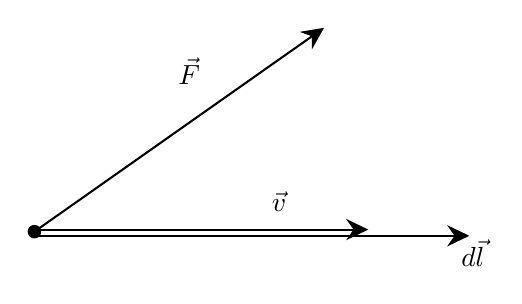
\begin{tikzpicture}[x=0.75pt,y=0.75pt,yscale=-1,xscale=1]
	%uncomment if require: \path (0,300); %set diagram left start at 0, and has height of 300

	%Shape: Circle [id:dp22141999262004308] 
	\draw  [fill={rgb, 255:red, 0; green, 0; blue, 0 }  ,fill opacity=1 ] (156.05,179.55) .. controls (156.05,178.03) and (157.28,176.8) .. (158.8,176.8) .. controls (160.32,176.8) and (161.55,178.03) .. (161.55,179.55) .. controls (161.55,181.07) and (160.32,182.3) .. (158.8,182.3) .. controls (157.28,182.3) and (156.05,181.07) .. (156.05,179.55) -- cycle ;
	%Straight Lines [id:da597861486650308] 
	\draw    (158.8,179.55) -- (295.88,83.06) ;
	\draw [shift={(298.33,81.33)}, rotate = 504.86] [fill={rgb, 255:red, 0; green, 0; blue, 0 }  ][line width=0.08]  [draw opacity=0] (10.72,-5.15) -- (0,0) -- (10.72,5.15) -- (7.12,0) -- cycle    ;
	%Straight Lines [id:da2655454358408562] 
	\draw    (158.8,181.55) -- (365.33,181.55) ;
	\draw [shift={(368.33,181.55)}, rotate = 180] [fill={rgb, 255:red, 0; green, 0; blue, 0 }  ][line width=0.08]  [draw opacity=0] (10.72,-5.15) -- (0,0) -- (10.72,5.15) -- (7.12,0) -- cycle    ;
	%Straight Lines [id:da9395712963407883] 
	\draw    (158.8,178.55) -- (316.67,178.55) ;
	\draw [shift={(319.67,178.55)}, rotate = 180] [fill={rgb, 255:red, 0; green, 0; blue, 0 }  ][line width=0.08]  [draw opacity=0] (10.72,-5.15) -- (0,0) -- (10.72,5.15) -- (7.12,0) -- cycle    ;

	% Text Node
	\draw (233.4,101.97) node    {$\vec{F}$};
	% Text Node
	\draw (276.73,165.3) node    {$\vec{v}$};
	% Text Node
	\draw (370.07,189.97) node    {$d\vec{l}$};

	\end{tikzpicture}
\end{figure}
\FloatBarrier

Supponiamo che tale spostamento avvenga in un intervallo di tempo $dt$. Chiamiamo il rapporto fra il lavoro compiuto dalla forza e l'intervallo di tempo in cui è stato compiuto \textbf{potenza dissipata dalla forza}. L'unità di misura della grandezza è $J/S$ e viene ribattezzata \emph{watt}. Possiamo esprimere la potenza come:

\[
	W=\frac{d\mathcal{L}}{dt}=\frac{\vec{F} \cdot d\vec{l}}{dt} = \vec{F} \cdot \vec{v}
\]

Consideriamo un conduttore di forma generica e concentriamoci su quello che accade in un istante infinitesimo. Le cariche si spostano entrambe della medesima quantità: chiamiamo dq la quantità di carica che attraversa la d.d.p. Per questo spostamento viene dissipata la potenza:

\[
	\boxed{W=\frac{d\mathcal{L}}{dt} = \frac{dQ\,\Delta V}{dt} = I\cdot \Delta V}
\]

Per i conduttori ohmici, quindi nel caso in cui vale la legge di Ohm, la potenza può anche essere riscritta come:

\[
	W=\frac{\Delta V^2}{R} = RI^2
\]

Questa legge che abbiamo trovato è detta \textbf{legge di Joule}. Essa mette in evidenza come il lavoro speso per far circolare la corrente elettrica sia necessario a vincere la resistenza opposta al reticolo cristallino al moto ordinario degli elettroni e, dal punto di vista termodinamico, esso viene assorbito dal conduttore la cui energia interna aumenta. Di conseguenza aumenta la temperatura del conduttore: se esso è isolato termicamente dall'ambiente circostante il processo porta alla fusione del metallo; se invece il conduttore è in contatto termico con l'ambiente, la sua temperatura cresce fino a che si raggiunge uno stato di equilibrio in cui l'energia interna non varia più e il lavoro elettrico viene ceduto all'ambiente sotto forma di calore (perché naturalmente la temperatura di equilibrio sia inferiore alla temperatura di fusione del conduttore). L'effetto di riscaldamento di un conduttore percorso da corrente si chiama \textbf{effetto Joule}.
I portatori di carica urtano in modo anaelastico con gli ioni del reticolo cristallino, che si scalda. Questo processo è quello che noi chiamiamo effetto Joule.

La relazione integrale $ W=\Delta V\cdot I $ si può anche estendere al caso microscopico.
Immaginiamo di avere un grande oggetto conduttore e di considerare al suo interno un campo elettrico.
Vogliamo studiare quello che accade in un istante infinitesimo. Immaginiamo di prendere una piccola porzione di conduttore. Vogliamo che il suo volume sia $d\tau$.

\begin{figure}[htpb]
	\centering

	\tikzset{every picture/.style={line width=0.75pt}} %set default line width to 0.75pt        

	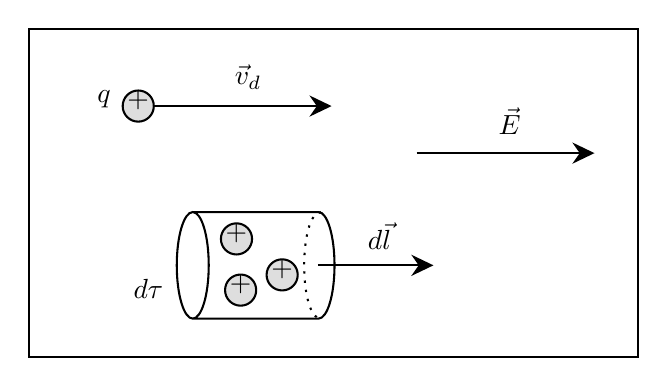
\begin{tikzpicture}[x=0.75pt,y=0.75pt,yscale=-1,xscale=1]
	%uncomment if require: \path (0,300); %set diagram left start at 0, and has height of 300

	%Shape: Can [id:dp757877143522663] 
	\draw   (254.03,131.67) -- (314.63,131.67) .. controls (318.89,131.67) and (322.33,143.16) .. (322.33,157.33) .. controls (322.33,171.51) and (318.89,183) .. (314.63,183) -- (254.03,183) .. controls (249.78,183) and (246.33,171.51) .. (246.33,157.33) .. controls (246.33,143.16) and (249.78,131.67) .. (254.03,131.67) .. controls (258.29,131.67) and (261.73,143.16) .. (261.73,157.33) .. controls (261.73,171.51) and (258.29,183) .. (254.03,183) ;
	%Curve Lines [id:da3467365634870494] 
	\draw  [dash pattern={on 0.84pt off 2.51pt}]  (315.76,131.67) .. controls (305.13,131.98) and (304.92,182.69) .. (315.76,183) ;
	%Shape: Circle [id:dp9534971715270861] 
	\draw  [fill={rgb, 255:red, 222; green, 222; blue, 222 }  ,fill opacity=1 ] (220.27,80.6) .. controls (220.27,76.46) and (223.62,73.1) .. (227.77,73.1) .. controls (231.91,73.1) and (235.27,76.46) .. (235.27,80.6) .. controls (235.27,84.74) and (231.91,88.1) .. (227.77,88.1) .. controls (223.62,88.1) and (220.27,84.74) .. (220.27,80.6) -- cycle ;

	%Straight Lines [id:da8479493413613088] 
	\draw    (235.27,80.6) -- (317.93,80.6) ;
	\draw [shift={(320.93,80.6)}, rotate = 180] [fill={rgb, 255:red, 0; green, 0; blue, 0 }  ][line width=0.08]  [draw opacity=0] (10.72,-5.15) -- (0,0) -- (10.72,5.15) -- (7.12,0) -- cycle    ;
	%Straight Lines [id:da33699563020269463] 
	\draw    (361.93,103.27) -- (444.6,103.27) ;
	\draw [shift={(447.6,103.27)}, rotate = 180] [fill={rgb, 255:red, 0; green, 0; blue, 0 }  ][line width=0.08]  [draw opacity=0] (10.72,-5.15) -- (0,0) -- (10.72,5.15) -- (7.12,0) -- cycle    ;
	%Shape: Rectangle [id:dp5473248941985187] 
	\draw   (175,43.33) -- (468.33,43.33) -- (468.33,201.33) -- (175,201.33) -- cycle ;
	%Straight Lines [id:da8728669115931522] 
	\draw    (314.33,157.33) -- (367,157.33) ;
	\draw [shift={(370,157.33)}, rotate = 180] [fill={rgb, 255:red, 0; green, 0; blue, 0 }  ][line width=0.08]  [draw opacity=0] (10.72,-5.15) -- (0,0) -- (10.72,5.15) -- (7.12,0) -- cycle    ;
	%Shape: Circle [id:dp291256225043645] 
	\draw  [fill={rgb, 255:red, 222; green, 222; blue, 222 }  ,fill opacity=1 ] (267.6,144.6) .. controls (267.6,140.46) and (270.96,137.1) .. (275.1,137.1) .. controls (279.24,137.1) and (282.6,140.46) .. (282.6,144.6) .. controls (282.6,148.74) and (279.24,152.1) .. (275.1,152.1) .. controls (270.96,152.1) and (267.6,148.74) .. (267.6,144.6) -- cycle ;

	%Shape: Circle [id:dp8259031963097847] 
	\draw  [fill={rgb, 255:red, 222; green, 222; blue, 222 }  ,fill opacity=1 ] (289.6,161.93) .. controls (289.6,157.79) and (292.96,154.43) .. (297.1,154.43) .. controls (301.24,154.43) and (304.6,157.79) .. (304.6,161.93) .. controls (304.6,166.08) and (301.24,169.43) .. (297.1,169.43) .. controls (292.96,169.43) and (289.6,166.08) .. (289.6,161.93) -- cycle ;

	%Shape: Circle [id:dp6700087166522872] 
	\draw  [fill={rgb, 255:red, 222; green, 222; blue, 222 }  ,fill opacity=1 ] (269.6,169.27) .. controls (269.6,165.12) and (272.96,161.77) .. (277.1,161.77) .. controls (281.24,161.77) and (284.6,165.12) .. (284.6,169.27) .. controls (284.6,173.41) and (281.24,176.77) .. (277.1,176.77) .. controls (272.96,176.77) and (269.6,173.41) .. (269.6,169.27) -- cycle ;

	% Text Node
	\draw (227.77,78.1) node    {$+$};
	% Text Node
	\draw (211.33,77.33) node    {$q$};
	% Text Node
	\draw (280.67,66.67) node    {$\vec{v}_{d}$};
	% Text Node
	\draw (406.67,88) node    {$\vec{E}$};
	% Text Node
	\draw (232.67,168.67) node    {$d\tau $};
	% Text Node
	\draw (344,143.33) node    {$d\vec{l}$};
	% Text Node
	\draw (275.1,142.1) node    {$+$};
	% Text Node
	\draw (297.1,159.43) node    {$+$};
	% Text Node
	\draw (277.1,166.77) node    {$+$};

	\end{tikzpicture}
\end{figure}
\FloatBarrier

Calcoliamo quanto vale il lavoro delle forze elettriche per spostare nell'istante $dt$ tutte le cariche del volumetto di uno spostamento $dl$.

\begin{align*}
	d\mathcal{L}^{(d\tau )} &= q\vec{E} \cdot d\vec{l} \, n \, d\tau \\
	d\mathcal{L}^{(d\tau )} &= q\vec{E} \underbrace{\vec{v}_ddt}_{d\vec{l}} \, n \, d\tau = \vec{E} \cdot \vec{J} \, dt \, d\tau \\
	dW^{(d\tau )} &= \frac{d\mathcal{L}^{(d\tau )}}{dt}= \frac{\vec{E} \cdot \vec{J} \, dt \, d\tau}{dt} = \vec{E} \cdot \vec{J}  \, d\tau
\end{align*}

E possiamo definire la \textbf{potenza dissipata per unità di volume}

\[
	\boxed{w = \frac{dW^{(d\tau )}}{d\tau} = \vec{E}  \cdot  \vec{J}}
\]

Se nello specifico stiamo considerando un conduttore ohmico avremo

\begin{gather*}
	\vec{J} = \sigma \vec{E}  \implies  w = \sigma E^2 \\
	\vec{E} = \rho \vec{J}  \implies  w = \rho J^2
\end{gather*}

\section{Forza elettromotrice}

Il regime stazionario corrisponde all'equazione $ \text{div}\vec{J} =0 $.
Quando un campo ha questa proprietà, è detto \textbf{solenoidale}. In questi casi non ci sono sorgenti di linee di flusso. Esse non possono essere altro che delle linee chiuse. Il campo elettrico non è solenoidale perché vi sono sempre da qualche parte delle sorgenti, punti in cui la divergenza non è nulla. Per avere il regime stazionario, dobbiamo avere un percorso conduttivo in cui le linee di flusso descrivono dei percorsi chiusi.

\begin{figure}[htpb]
	\centering

	\tikzset{every picture/.style={line width=0.75pt}} %set default line width to 0.75pt        

	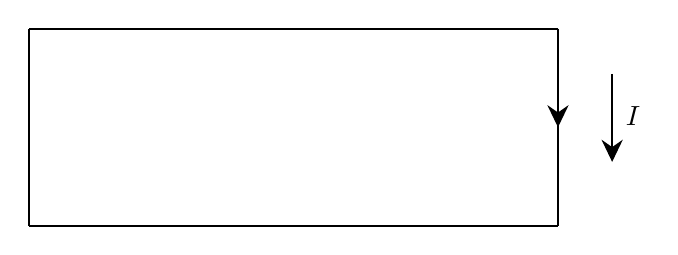
\begin{tikzpicture}[x=0.75pt,y=0.75pt,yscale=-1,xscale=1]
	%uncomment if require: \path (0,300); %set diagram left start at 0, and has height of 300

	%Straight Lines [id:da9476843193458615] 
	\draw    (402.5,46) -- (402.5,141) ;
	\draw [shift={(402.5,93.5)}, rotate = 270] [fill={rgb, 255:red, 0; green, 0; blue, 0 }  ][line width=0.08]  [draw opacity=0] (10.72,-5.15) -- (0,0) -- (10.72,5.15) -- (7.12,0) -- cycle    ;
	%Straight Lines [id:da614935104864186] 
	\draw    (402.5,46) -- (147.5,46) ;
	%Straight Lines [id:da07877041729371093] 
	\draw    (402.5,141) -- (147.5,141) ;
	%Straight Lines [id:da5055683085293592] 
	\draw    (147.5,46) -- (147.5,141) ;
	%Straight Lines [id:da5941319138495598] 
	\draw    (428.6,67.77) -- (428.6,107.17) ;
	\draw [shift={(428.6,110.17)}, rotate = 270] [fill={rgb, 255:red, 0; green, 0; blue, 0 }  ][line width=0.08]  [draw opacity=0] (10.72,-5.15) -- (0,0) -- (10.72,5.15) -- (7.12,0) -- cycle    ;

	% Text Node
	\draw (438.67,88.22) node    {$I$};

	\end{tikzpicture}
\end{figure}
\FloatBarrier

Per la legge di Ohm in forma integrale applicata ad un circuito chiuso, sappiamo che:

\[
	\oint_{\gamma} \vec{E} \cdot d\vec{l} = R_t i
\]

Dove $ R_t  $ è la resistenza totale del circuito stesso. Vediamo come il processo di conduzione stazionario sia un processo dissipativo. Il lavoro per condurre la carica lungo il circuito non sarà nullo. Potremmo chiederci quale è la forza che compie questo lavoro, Ogni carica che scorre nel circuito è sottoposto ad una forza elettrica.
Tuttavia, dal momento che E è conservativo, si ha che:

\[
	\mathcal{L} =\oint_{\gamma} \vec{E} \cdot d\vec{l} = \oint_{\gamma} q\vec{E} \cdot d\vec{l} =0
\]

Il campo elettrico non può compiere lavoro su un percorso chiuso con una conseguente impossibilità di sostenere un processo di conduzione stazionario.
La circolazione delle cariche attraverso il circuito è garantita dal generatore di forza elettromotrice, che ha al suo interno delle forze di natura non elettrostatica, non conservative, che possono determinare il moto continuo delle cariche.

\begin{figure}[htpb]
	\centering

	\tikzset{every picture/.style={line width=0.75pt}} %set default line width to 0.75pt        

	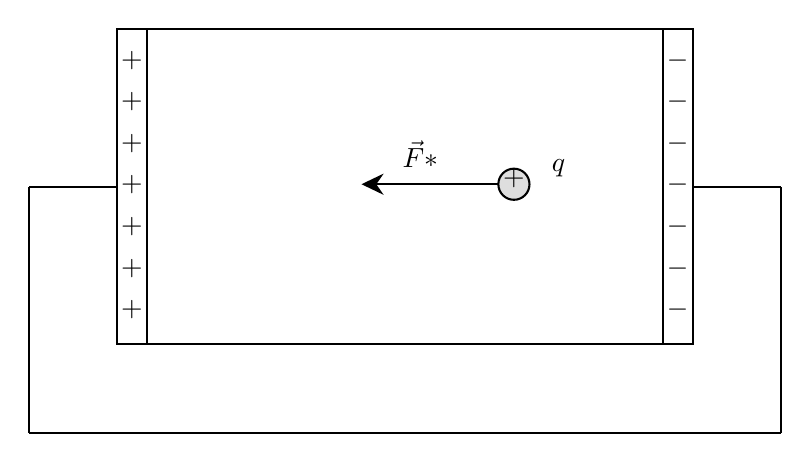
\begin{tikzpicture}[x=0.75pt,y=0.75pt,yscale=-1,xscale=1]
	%uncomment if require: \path (0,300); %set diagram left start at 0, and has height of 300

	%Straight Lines [id:da9462970824287664] 
	\draw    (474.5,119.33) -- (474.5,238) ;
	%Straight Lines [id:da005797569061894325] 
	\draw    (154.5,119.33) -- (112,119.33) ;
	%Straight Lines [id:da6061661728139769] 
	\draw    (474.5,238) -- (112,238) ;
	%Straight Lines [id:da6122974189521297] 
	\draw    (112,119.33) -- (112,238) ;
	%Shape: Rectangle [id:dp03509844529887096] 
	\draw   (169,43) -- (417.5,43) -- (417.5,195) -- (169,195) -- cycle ;
	%Shape: Rectangle [id:dp2522424612146723] 
	\draw   (169,43) -- (154.5,43) -- (154.5,195) -- (169,195) -- cycle ;
	%Shape: Rectangle [id:dp11615323912801867] 
	\draw   (432,43) -- (417.5,43) -- (417.5,195) -- (432,195) -- cycle ;
	%Straight Lines [id:da33287730947959715] 
	\draw    (474.5,119.33) -- (432,119.33) ;
	%Shape: Circle [id:dp16159178135504249] 
	\draw  [fill={rgb, 255:red, 222; green, 222; blue, 222 }  ,fill opacity=1 ] (338.27,117.93) .. controls (338.27,113.79) and (341.62,110.43) .. (345.77,110.43) .. controls (349.91,110.43) and (353.27,113.79) .. (353.27,117.93) .. controls (353.27,122.08) and (349.91,125.43) .. (345.77,125.43) .. controls (341.62,125.43) and (338.27,122.08) .. (338.27,117.93) -- cycle ;

	%Straight Lines [id:da9308438901155345] 
	\draw    (338.27,117.93) -- (275.33,117.93) ;
	\draw [shift={(272.33,117.93)}, rotate = 360] [fill={rgb, 255:red, 0; green, 0; blue, 0 }  ][line width=0.08]  [draw opacity=0] (10.72,-5.15) -- (0,0) -- (10.72,5.15) -- (7.12,0) -- cycle    ;

	% Text Node
	\draw (161.67,58.33) node    {$+$};
	% Text Node
	\draw (161.67,78.33) node    {$+$};
	% Text Node
	\draw (161.67,98.33) node    {$+$};
	% Text Node
	\draw (161.67,118.33) node    {$+$};
	% Text Node
	\draw (161.67,138.33) node    {$+$};
	% Text Node
	\draw (161.67,158.33) node    {$+$};
	% Text Node
	\draw (161.67,178.33) node    {$+$};
	% Text Node
	\draw (424.67,58.33) node    {$-$};
	% Text Node
	\draw (424.67,78.33) node    {$-$};
	% Text Node
	\draw (424.67,98.33) node    {$-$};
	% Text Node
	\draw (424.67,118.33) node    {$-$};
	% Text Node
	\draw (424.67,138.33) node    {$-$};
	% Text Node
	\draw (424.67,158.33) node    {$-$};
	% Text Node
	\draw (424.67,178.33) node    {$-$};
	% Text Node
	\draw (367.33,110) node    {$q$};
	% Text Node
	\draw (345.77,115.43) node    {$+$};
	% Text Node
	\draw (300.67,103.33) node    {$\vec{F} *$};

	\end{tikzpicture}
\end{figure}
\FloatBarrier

Esso, grazie a queste forze, sposta delle cariche da un lato all'altro accumulando su estremo carica positiva e su un altro carica negativa. Produrrà all'interno del circuito un campo elettrico e quando le cariche arrivano ad un suo estremo, il generatore le porta all'estremo successivo. Per comprendere questo meccanismo, introduciamo un nuovo campo vettoriale nel generatore, detto \textbf{campo elettromotore}, pari al rapporto fra la forza non conservativa che trasferiamo all'interno del conservatore e la carica su cui questa forza agisce. Si tratta sempre di un campo elettrico coulombiano, si misura con la stessa unità di misura. Chiamiamo i due estremi del generatore poli.

\subsection{Generatore a circuito aperto}

Quando il generatore è staccato dal conduttore esterno, mano a mano che accumulo cariche sui poli, esse producono un campo elettrostatico in aumento, diretto dalle cariche positive verso quelle negative.

\begin{figure}[htpb]
	\centering

	\tikzset{every picture/.style={line width=0.75pt}} %set default line width to 0.75pt        

	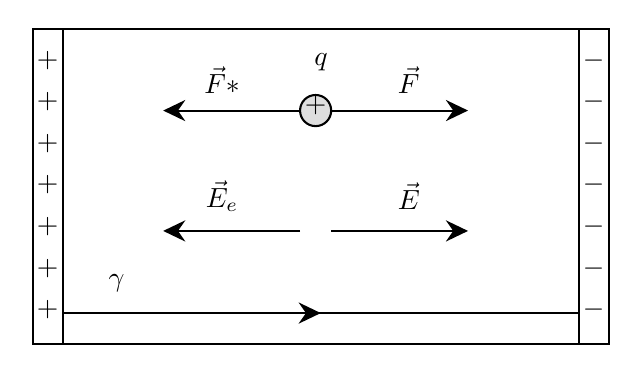
\begin{tikzpicture}[x=0.75pt,y=0.75pt,yscale=-1,xscale=1]
	%uncomment if require: \path (0,300); %set diagram left start at 0, and has height of 300

	%Shape: Rectangle [id:dp5181084226757073] 
	\draw   (170,75) -- (418.5,75) -- (418.5,227) -- (170,227) -- cycle ;
	%Shape: Rectangle [id:dp08607693266497796] 
	\draw   (170,75) -- (155.5,75) -- (155.5,227) -- (170,227) -- cycle ;
	%Shape: Rectangle [id:dp8799864593554507] 
	\draw   (433,75) -- (418.5,75) -- (418.5,227) -- (433,227) -- cycle ;
	%Shape: Circle [id:dp1343846334943457] 
	\draw  [fill={rgb, 255:red, 222; green, 222; blue, 222 }  ,fill opacity=1 ] (284.27,114.43) .. controls (284.27,110.29) and (287.62,106.93) .. (291.77,106.93) .. controls (295.91,106.93) and (299.27,110.29) .. (299.27,114.43) .. controls (299.27,118.58) and (295.91,121.93) .. (291.77,121.93) .. controls (287.62,121.93) and (284.27,118.58) .. (284.27,114.43) -- cycle ;

	%Straight Lines [id:da9326497794989177] 
	\draw    (284.27,114.43) -- (221.33,114.43) ;
	\draw [shift={(218.33,114.43)}, rotate = 360] [fill={rgb, 255:red, 0; green, 0; blue, 0 }  ][line width=0.08]  [draw opacity=0] (10.72,-5.15) -- (0,0) -- (10.72,5.15) -- (7.12,0) -- cycle    ;
	%Straight Lines [id:da5145606566488408] 
	\draw    (418.5,212) -- (170,212) ;
	\draw [shift={(294.25,212)}, rotate = 180] [fill={rgb, 255:red, 0; green, 0; blue, 0 }  ][line width=0.08]  [draw opacity=0] (10.72,-5.15) -- (0,0) -- (10.72,5.15) -- (7.12,0) -- cycle    ;
	%Straight Lines [id:da05978377752574082] 
	\draw    (362.2,114.43) -- (299.27,114.43) ;
	\draw [shift={(365.2,114.43)}, rotate = 180] [fill={rgb, 255:red, 0; green, 0; blue, 0 }  ][line width=0.08]  [draw opacity=0] (10.72,-5.15) -- (0,0) -- (10.72,5.15) -- (7.12,0) -- cycle    ;
	%Straight Lines [id:da06615514171888282] 
	\draw    (284.27,172.43) -- (221.33,172.43) ;
	\draw [shift={(218.33,172.43)}, rotate = 360] [fill={rgb, 255:red, 0; green, 0; blue, 0 }  ][line width=0.08]  [draw opacity=0] (10.72,-5.15) -- (0,0) -- (10.72,5.15) -- (7.12,0) -- cycle    ;
	%Straight Lines [id:da5274416088289138] 
	\draw    (362.2,172.43) -- (299.27,172.43) ;
	\draw [shift={(365.2,172.43)}, rotate = 180] [fill={rgb, 255:red, 0; green, 0; blue, 0 }  ][line width=0.08]  [draw opacity=0] (10.72,-5.15) -- (0,0) -- (10.72,5.15) -- (7.12,0) -- cycle    ;

	% Text Node
	\draw (162.67,90.33) node    {$+$};
	% Text Node
	\draw (162.67,110.33) node    {$+$};
	% Text Node
	\draw (162.67,130.33) node    {$+$};
	% Text Node
	\draw (162.67,150.33) node    {$+$};
	% Text Node
	\draw (162.67,170.33) node    {$+$};
	% Text Node
	\draw (162.67,190.33) node    {$+$};
	% Text Node
	\draw (162.67,210.33) node    {$+$};
	% Text Node
	\draw (425.67,90.33) node    {$-$};
	% Text Node
	\draw (425.67,110.33) node    {$-$};
	% Text Node
	\draw (425.67,130.33) node    {$-$};
	% Text Node
	\draw (425.67,150.33) node    {$-$};
	% Text Node
	\draw (425.67,170.33) node    {$-$};
	% Text Node
	\draw (425.67,190.33) node    {$-$};
	% Text Node
	\draw (425.67,210.33) node    {$-$};
	% Text Node
	\draw (294.33,91) node    {$q$};
	% Text Node
	\draw (246.67,99.83) node    {$\vec{F} *$};
	% Text Node
	\draw (291.77,111.93) node    {$+$};
	% Text Node
	\draw (195.83,197.5) node    {$\gamma $};
	% Text Node
	\draw (336.67,99.83) node    {$\vec{F}$};
	% Text Node
	\draw (246.67,155.83) node    {$\vec{E}_{e}$};
	% Text Node
	\draw (336.67,155.83) node    {$\vec{E}$};

	\end{tikzpicture}
\end{figure}
\FloatBarrier

A questo punto sulla carica agiscono due forze: la forza non conservativa e quella coulombiana che tende a respingere la carica. In regime stazionario arriviamo a una situazione di equilibrio in cui la risultante delle forze agenti sulla carica diventerà pari a zero. Questa situazione è dovuta al fatto che l'accumulo di carica sui poli impedisce un ulteriore spostamento di carica (per repulsione elettrostatica).

\[
	\vec{R} = \vec{F} + \vec{F}^* = 0 \qquad q(\vec{E} +\vec{E}_e ) = 0\implies \vec{E} = - \vec{E}_e
\]

Consideriamo un percorso $\gamma$ che va dal polo positivo al polo negativo. Calcoliamoci l'integrale di linea lungo il percorso nei due casi:

\begin{gather*}
	\int_{A,\gamma}^B \vec{E} \cdot d\vec{l} = - \int_A^B \vec{E}_e \cdot d\vec{l} \\
	V_A-V_B = \Delta V = \int_{B,\gamma}^A \vec{E}_e\cdot d\vec{l} = f \\
	\boxed{V_A-V_B=fem}
\end{gather*}

Ciò che abbiamo ottenuto è detta forza elettromotrice ($fem$). Non si tratta tuttavia di una forza, ha le dimensioni di un potenziale ed è proprio la d.d.p. misurata ai capi del generatore a circuito aperto.

\subsection{Generatore a circuito chiuso}

Proviamo a collegare il generatore a un circuito. Esso provoca la circolazione di corrente. Sulla carica all'interno del generatore agiranno entrambi i campi sopra definiti.

\begin{figure}[htpb]
	\centering

	\tikzset{every picture/.style={line width=0.75pt}} %set default line width to 0.75pt        

	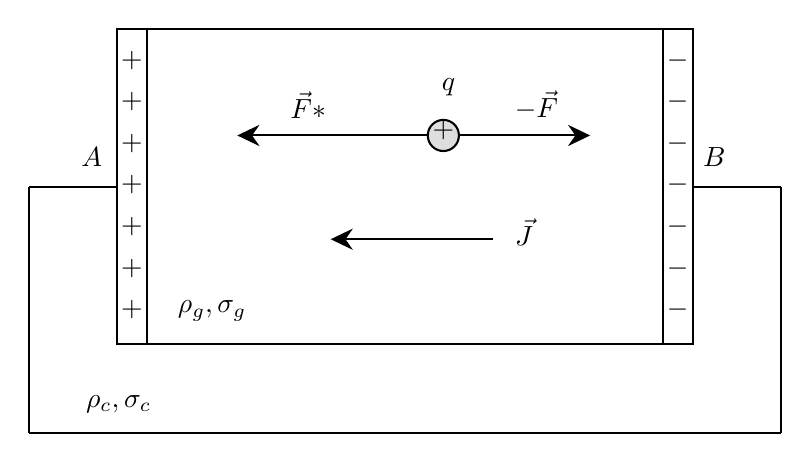
\begin{tikzpicture}[x=0.75pt,y=0.75pt,yscale=-1,xscale=1]
	%uncomment if require: \path (0,300); %set diagram left start at 0, and has height of 300

	%Straight Lines [id:da6043179485749723] 
	\draw    (494.5,139.33) -- (494.5,258) ;
	%Straight Lines [id:da10221033382838973] 
	\draw    (174.5,139.33) -- (132,139.33) ;
	%Straight Lines [id:da6558814232584502] 
	\draw    (494.5,258) -- (132,258) ;
	%Straight Lines [id:da62131025025839] 
	\draw    (132,139.33) -- (132,258) ;
	%Shape: Rectangle [id:dp0952509793199432] 
	\draw   (189,63) -- (437.5,63) -- (437.5,215) -- (189,215) -- cycle ;
	%Shape: Rectangle [id:dp16008206437810846] 
	\draw   (189,63) -- (174.5,63) -- (174.5,215) -- (189,215) -- cycle ;
	%Shape: Rectangle [id:dp7768738225428726] 
	\draw   (452,63) -- (437.5,63) -- (437.5,215) -- (452,215) -- cycle ;
	%Straight Lines [id:da8208347839397301] 
	\draw    (494.5,139.33) -- (452,139.33) ;
	%Shape: Circle [id:dp33343919986697257] 
	\draw  [fill={rgb, 255:red, 222; green, 222; blue, 222 }  ,fill opacity=1 ] (324.27,114.43) .. controls (324.27,110.29) and (327.62,106.93) .. (331.77,106.93) .. controls (335.91,106.93) and (339.27,110.29) .. (339.27,114.43) .. controls (339.27,118.58) and (335.91,121.93) .. (331.77,121.93) .. controls (327.62,121.93) and (324.27,118.58) .. (324.27,114.43) -- cycle ;

	%Straight Lines [id:da053558009454149236] 
	\draw    (324.27,114.43) -- (235.5,114.43) ;
	\draw [shift={(232.5,114.43)}, rotate = 360] [fill={rgb, 255:red, 0; green, 0; blue, 0 }  ][line width=0.08]  [draw opacity=0] (10.72,-5.15) -- (0,0) -- (10.72,5.15) -- (7.12,0) -- cycle    ;
	%Straight Lines [id:da19431546395832155] 
	\draw    (399.5,114.43) -- (339.27,114.43) ;
	\draw [shift={(402.5,114.43)}, rotate = 180] [fill={rgb, 255:red, 0; green, 0; blue, 0 }  ][line width=0.08]  [draw opacity=0] (10.72,-5.15) -- (0,0) -- (10.72,5.15) -- (7.12,0) -- cycle    ;
	%Straight Lines [id:da6578194814557985] 
	\draw    (355.5,164.43) -- (280.5,164.43) ;
	\draw [shift={(277.5,164.43)}, rotate = 360] [fill={rgb, 255:red, 0; green, 0; blue, 0 }  ][line width=0.08]  [draw opacity=0] (10.72,-5.15) -- (0,0) -- (10.72,5.15) -- (7.12,0) -- cycle    ;

	% Text Node
	\draw (181.67,78.33) node    {$+$};
	% Text Node
	\draw (181.67,98.33) node    {$+$};
	% Text Node
	\draw (181.67,118.33) node    {$+$};
	% Text Node
	\draw (181.67,138.33) node    {$+$};
	% Text Node
	\draw (181.67,158.33) node    {$+$};
	% Text Node
	\draw (181.67,178.33) node    {$+$};
	% Text Node
	\draw (181.67,198.33) node    {$+$};
	% Text Node
	\draw (444.67,78.33) node    {$-$};
	% Text Node
	\draw (444.67,98.33) node    {$-$};
	% Text Node
	\draw (444.67,118.33) node    {$-$};
	% Text Node
	\draw (444.67,138.33) node    {$-$};
	% Text Node
	\draw (444.67,158.33) node    {$-$};
	% Text Node
	\draw (444.67,178.33) node    {$-$};
	% Text Node
	\draw (444.67,198.33) node    {$-$};
	% Text Node
	\draw (334.33,91) node    {$q$};
	% Text Node
	\draw (266.67,99.83) node    {$\vec{F} *$};
	% Text Node
	\draw (376.67,99.83) node    {$-\vec{F}$};
	% Text Node
	\draw (331.77,111.93) node    {$+$};
	% Text Node
	\draw (162.33,125) node    {$A$};
	% Text Node
	\draw (462.33,125) node    {$B$};
	% Text Node
	\draw (220.33,199) node    {$\rho _{g} ,\sigma _{g}$};
	% Text Node
	\draw (175.33,244) node    {$\rho _{c} ,\sigma _{c}$};
	% Text Node
	\draw (370.67,160.83) node    {$\vec{J}$};

	\end{tikzpicture}
\end{figure}
\FloatBarrier

Essi non possono più essere uguali e opposti perché se lo fossero le cariche non si sposterebbero. È necessario che la forza non conservativa vinca sulla forza di repulsione elettrostatica. Il campo elettromotore in modulo deve diventare maggiore del campo elettrico:

\[
	|\vec{E}_e| > |\vec{E}|
\]

Sappiamo che al conduttore viene sempre associata una resistività $ \rho_c  $, tale che:

\[
	\vec{E} = \rho_c\vec{J} \qquad \vec{J} =\sigma_c\vec{E}
\]

Anche il generatore ha una resistività interna caratteristica che possiamo definire come:

\[
	\boxed{(\vec{E} +\vec{E}_e ) = \rho_g\vec{J} \qquad \vec{J} = \sigma_g (\vec{E} + \vec{E}_e )}
\]

Tale relazione prende il nome di \emph{legge di Ohm generalizzata}, perché viene estesa all'interno del generatore.

\begin{align*}
	\underbrace{\int_{A,\gamma}^B \vec{E} \cdot d\vec{l}}_{\Delta V} + \int_{A,\gamma}^B \vec{E}_e\cdot d\vec{l} &= \int_A^B \rho_g \vec{J} \cdot d\vec{l}\\
	\Delta V &= - \int_{A,\gamma}^B \vec{E}_e\cdot d\vec{l} + \int_A^B \rho_g \vec{J} \cdot d\vec{l} \\
	\Delta V &= \underbrace{\int_{B,\gamma}^A \vec{E}_e\cdot d\vec{l}}_{fem} + \underbrace{\int_A^B \rho_g \vec{J} \cdot d\vec{l}}_{<0} \\
\end{align*}

La quantità con nel secondo integrale è pari a:

\[
	\int_A^B \rho_g \vec{J} \cdot d\vec{l} = \int_A^B \rho_g \frac{I}{S} dl = -I \underbrace{\rho_g\frac{l}{S}}_r = -Ir
\]

Si ottiene allora:

\[
	\boxed{\Delta V = fem - rI}
\]

La relazione esprime come parte della capacità di spostare cariche serve per vincere la resistenza, tutto il resto è differenza di potenziale ai lati disponibile.

Dal momento che il generatore oltre alla $fem$ ha anche resistenza interna, si schematizza un generatore reale come un generatore ideale in serie con una resistenza interna. Questo oggetto viene poi collegato al resistore esterno.